\documentclass[a4paper, 11pt, titlepage]{article}
\usepackage{fancyhdr}
\usepackage{graphicx}
\usepackage{imakeidx}
\usepackage{makeidx}
\usepackage{mathtools}
\usepackage[spanish]{babel}
\usepackage{eurosym}
\usepackage{hyperref}

% CODE C
\usepackage{amssymb}
\usepackage{listings}
\usepackage{xcolor}
\definecolor{textblue}{rgb}{.2,.2,.7}
\definecolor{textred}{rgb}{0.54,0,0}
\definecolor{textgreen}{rgb}{0,0.43,0}
\lstset{
numberstyle=\tiny, 
stepnumber=1,
numbersep=5pt, 
tabsize=4,
basicstyle=\ttfamily,
keywordstyle=\color{textblue},
commentstyle=\color{textred},   
stringstyle=\color{textgreen},
frame=none,                    
columns=fullflexible,
keepspaces=true,
xleftmargin=\parindent,
showstringspaces=false}

\lstset{basicstyle=\ttfamily,
    showstringspaces=false,
    commentstyle=\color{red},
    keywordstyle=\color{blue}
}

\setcounter{secnumdepth}{5}
\setcounter{tocdepth}{5}

\title{Programación C en el entorno *nix}
\author{Francisco Javier Balón Aguilar}

\begin{document}

\maketitle
\renewcommand{\contentsname}{Índice}
\tableofcontents
\newpage

\section{Breve contextualización}

    Un conjunto de instrucciones que pueden ser ejecutadas en una CPU, junto con su 
    sistema de codificación se denomina \textbf{lenguaje máquina}.

    Este lenguaje puede ser considerado como el primer lenguaje de programación, y 
    es entendido directamente por el ordenador aunque, al estar íntimamente 
    unido a la estructura y circuitería del computador, su uso queda muy alejado de 
    la forma en que se suelen expresar los problemas matemáticos y lógicos comunes.

    Las principales características del lenguaje máquina son:

    \begin{itemize}
        \item Las instrucciones están formadas por cadenas binarias (0 y 1).
        \item Los datos se manejan a través de direcciones de memoria donde se encuentran
        almacenados, sin admitir identificadores. Es el propio programador el que debe 
        realizar la asignación de direcciones de memoria para todas las variables y 
        constantes del programa.
        \item Las instrucciones sólo realizan operaciones muy simples, dependientes de 
        la circuitería interna del procesador.
    \end{itemize}

    En los inicios de la informática, el programador se comunicaba con el ordenador 
    por medio del conexionado de cableado; lo que posteriormente dió lugar a la 
    comunicación mediante números binarios. Estas tareas resultaban engorrosas y pesadas, 
    por lo que pronto se inventarían las notaciones simbólicas\footnote{
        Las notaciones son palabras clave que el programa traduciría automáticamente 
        a su versión binaria. De forma que el programador debe recordar una palabra
        y no un conjunto de 0s y 1s.

        Por ejemplo, el programador escribe la instrucción:

        \[MOV B , M(7)\]

        Y el programa traductor lo convierte internamente a:

        \[000100100000\]

        Lo que provocaría que el ordenador mueva al registro $B$ el contenido de la posición 
        de memoria $7$.
    }.

    El programa traductor se conoce como \textbf{ensamblador}, y el lenguaje simbólico
    que se utiliza para ello es conocido como \textbf{lenguaje ensamblador}. Este 
    lenguaje requiere que el programador escriba una línea por cada una de las 
    instrucciones que realizará la máquina.

    Como se observa, ambos lenguajes fuerzan al programador a pensar directamente en 
    la estructura propia de  la máquina a la hora de realizar cualquier programa.
    Aunque la aparición de los lenguajes ensambladores fue importante, y un paso en 
    la simplificación -recordemos que veníamos del lenguaje máquina-, la tarea de 
    programación seguíasiendo ardua (y sigue siéndolo en la actualidad en estos 
    lenguajes).

    Para solucionar y mejorar la eficiencia de la programación se desarrollaron los 
    denominados \textbf{lenguajes de alto nivel}, teniendo estos una sintaxis y una
    escritura más amistosa para el humano y centrándose más en la forma de pensar 
    para resolver los problemas independientemente de la máquina.

    El lenguaje C es un lenguaje de alto nivel, considerado un \textbf{pura sangre}
    por muchos programadores, ya que los programas escritos en C producen un código 
    especialmente veloz y eficiente, pues con él se puede hacer prácticamente todo 
    lo que su hardware permite realizar.

    Fue desarrollado por \textit{Dennis Ritchie}\footnote{
        \textit{Dennis Ritchie} tiene además la importante paternidad, junto a 
        \textit{Ken Thompson}, del sistema 
        operativo UNIX. De hecho, C y UNIX se encuentran íntimamente unidos.
        También fue coautor junto a \textit{Brian Kernighan} del manual 
        \textit{El lenguaje de programación C}, que durante años fue el estándar 
        de facto del lenguaje (K\&R C), hasta la aparición del ANSI C (para el que 
        apareció la segunda edición de \textit{El lenguaje de Programación C}).
    } a principios de la década de los 70 en \textit{Bell Labs}.

    C nace como evolución natural del lenguaje B (de ahí su nombre).

    \subsection{Filosofía}

        Uno de los objetivos de diseño del lenguaje C es que solo sean necesarias 
        unas pocas instrucciones en lenguaje máquina para traducir cada elemento 
        del lenguaje, sin que haga falta un soporte intenso en tiempo de ejecución. 
        Es muy posible escribir C a bajo nivel de abstracción; de hecho, C se usó 
        como intermediario entre diferentes lenguajes.

        En parte, a causa de ser de relativamente bajo nivel y de tener un modesto 
        conjunto de características, se pueden desarrollar compiladores de C fácilmente. 
        En consecuencia, el lenguaje C está disponible en un amplio abanico de 
        plataformas (más que cualquier otro lenguaje). Además, a pesar de su naturaleza 
        de bajo nivel, el lenguaje se desarrolló para incentivar la programación 
        independiente de la máquina. Un programa escrito cumpliendo los estándares e 
        intentando que sea portátil puede compilarse en muchos computadores.

        C se desarrolló originalmente (conjuntamente con el sistema operativo Unix, 
        con el que ha estado asociado mucho tiempo) por programadores para programadores. 
        Sin embargo, ha alcanzado una popularidad enorme, y se ha usado en contextos muy 
        alejados de la programación de software de sistema, para la que se diseñó 
        originalmente. 

\section{Hola mundo}

    Como es costumbre en la programación. El primer programa a escribir en un lenguaje es e
    el conocido como \textit{Hola mundo} o \textit{Hello world}.

    \begin{lstlisting}[language=C,numbers=left]
    #include <stdio.h>
    main()
    {
        printf("Hola mundo \n");
    }\end{lstlisting}

    La primera línea del programa, 

    \begin{lstlisting}[language=C]
        #include <stdio.h>\end{lstlisting}

    indica al compilador (véase sección \ref{compilador}) que incluya información 
    sobre la librería estándar \textit{input/output}. 
    
    Posteriormene definimos una función llamada \textit{main} que no recibe argumentos,

    \begin{lstlisting}[language=C]
        main() {}\end{lstlisting}

    siendo lo que encuentra entre las llaves el código de esta función, el cual,
    
    \begin{lstlisting}[language=C]
        printf("Hola mundo \n");\end{lstlisting}

    llama a la función \textit{printf}, que recibe como argumento una secuencia de caracteres,
    para ser impresos. Como nota adicional, el carácter $\backslash n$ indica un carácter 
    de salto de línea.

    Estos elementos se desarrollarán progresivamente en el presente documento.
    

\section{El compilador gcc}\label{compilador}

    Los compiladores de Unix han sido tan importantes que se han tomado como estándar para la industria 
    del software. Aunque existen varios compiladores, el más famoso en Linux es GNU gcc (Gnu Compiler 
    Collection). Escrito inicialmente por \textit{Richard Stallman} y \textit{Leonard H. Tower}.

    \begin{figure}[htp]
        \centering
        
\includegraphics[width=0.4\textwidth]{resources/gnu-gcc.png}
        \caption{Imagen dada al proyecto GNU gcc.}
        \label{gcclogo}
    \end{figure}

    gcc ha sido escrito inicialmente para C, aunque también admite C++ y dispone de frontends para 
    lenguajes diversos. gcc genera un código optimizado, reconociendo todos los estándares del lenguaje C
    y ANSI C; por esta razón es utilizado por diferentes IDEs como compilador base.

    A continuación vemos un sencillo código <<Hola mundo>> de lenguaje C.

    \begin{lstlisting}[language=C,numbers=left]
    #include <stdio.h>
    main()
    {
        printf("Hola mundo \n");
    }\end{lstlisting}

    Compilándolo con gcc obtendremos el binario ejecutable (\textit{./hola}).
    
    \begin{lstlisting}[language=bash]
    gcc -o hola hola.c\end{lstlisting}
        
    \subsection{Usos y parámetros básicos de gcc}

        Por supuesto para más información es recomendable leer la documentación oficial de GNU gcc\footnote{
            <<The GNU C Reference Manual>> por Trevis Rothwell y James Youngman. Alojado en el 
            servidor gnu.org/software/gnu-c-manual/gnu-c-manual.pdf.
        } y leer el manual \footnote{
            \textit{man gcc}
        }.

        No obstante observaremos algunas opciones y paráemtros empleados con frecuencia, por ejemplo para obtener 
        el ejecutable usando un estándar específico:

        \begin{lstlisting}[language=bash]
    # Estandar de 1999
    gcc -std=c99 -o hola hola.c

    # Estandar 2011
    gcc -std=c11 -o hola hola.c\end{lstlisting}

        Como ya hemos adelantado previamente, si usamos gcc con el parámetro $-o$ generará el binario con el nombre
        que le pasamos; en caso de no hacerlo generará un binario llamado por defecto \textit{./a.out}. 
        
        Si en vez de generar un binario queremos generar el código ensamblador correspondiente al código fuente 
        podemos hacerlo usando el parámetro $-S$. Esto generará un ASMen formato por defecto \textit{AT\&T}; si queremos
        especificar un formato concreto se lo añadimos:

        \begin{lstlisting}[language=bash]
    gcc -S hola.c               # Por defecto AT&T
    gcc -S -masm=att hola.c     # AT&T
    gcc -S -masm=Intel hola.c   # Intel\end{lstlisting}

        Podemos obtener un código objeto sin enlazar con $-c$. Si necesitamos incluir bibliotecas o ficheros de 
        cabecera (\textit{.h}) podemos usar los parámetros $-L$ o $-l$, respectivamente.
         
        \begin{lstlisting}[language=bash]
    gcc -c hola.c               # Codigo objeto
    gcc hola.c -Llib -o hola
    gcc -Iproyecto/src hola.c -o hola\end{lstlisting}

        Podemos además optimizar el binario para una microarquitectura de CPU concreta o para una familia en específico.

        \begin{lstlisting}[language=bash,basicstyle=\small]
    #Para una de estas familias o tipos de CPU
    gcc -m486 hola.c -o hola
    gcc -m386 hola.c -o hola
    
    #Para una CPU concreta (anteriormente -mcpu)
    gcc -mtune=k8 hola.c -o hola
    gcc -mtune=prescott hola.c -o hola
    gcc -mtune=athlon-4 hola.c -o hola
    
    #Para un tipo de FPU o extensiones especificas. 
    # Por ejemplo, para SSE
    gcc -mfpmath=sse hola.c -o hola
    
    #Tambien puedes combinar opciones, por ejemplo, 
    # para un nivel de optimizacion 3 y para AMD Zen 2
    gcc -O3 -march=znver2 hola.c -o hola \end{lstlisting}

    \subsection{Diferencia entre \textit{\#include \textless filename\textgreater} e \textit{\#include ``filename''}}

        Cuando utilizamos \textit{\#include \textless filename\textgreater}, estamos indicando al compilador
        que busque este encabezado en su directorio \textit{includes}. Podemos resumirlo en 
        que buscará este archivo en los propios archivos de C y el compilador.  

        Por el contrario, cuando utilizamos \textit{\#include ``filename"} le indicamos al compilador que busque
        este encabezado en el directorio actual (\textit{.}). Por ello es usado para los encabezados
        creados por el programador.

        \begin{lstlisting}[language=C,numbers=left]
    #include <stdio.h>
    #include "my_header.h"\end{lstlisting}

        Podemos usar el parámetro $-I$ de gcc para indicarle que, al encontrar una inclusión 
        entre \textit{\textless\textgreater} también debe buscar encabezados en el directorio 
        posterior al parámetro. De esta forma, gcc tratará al directorio parametrizado como 
        si se tratase del directorio \textit{includes}.
        
        \begin{lstlisting}[language=bash]
    gcc hola.c -I .\end{lstlisting}

\section{La herramienta make y el makefile}\label{make}

    Make es una herramienta de gestión de dependencias usada en entornos de la familia UNIX. 
    Es una buena práctica para compilar de forma automatizada códigos compuestos y complejos, 
    por ejemplo en códigos compuestos de códigos C en distintos ficheros con distintos ficheros
    de cabecera (\textit{.h}).

    Para preparar el funcionamiento de make es necesario crear un fichero, en el cual se especifica
    y se configura todo lo necesario para el proceso. Este fichero es denominado makefile. Podemos
    decir que son las instrucciones que make debe realizar.

    Como añadido, make entiende los formatos y extensiones, dando una respuesta apropiada a cada tipo
    de archivo.

    El formato genérico para un makefile es el siguiente:

    \begin{lstlisting}[language=make]
    VARIABLES
    ...
    
    OBJETIVO:  DEPENDENCIAS 
        COMANDO
        ...\end{lstlisting}

    Un makefile simple para realizar con make la compilación de un programa C sería similar al siguiente:

    \begin{lstlisting}[language=make]
    hola:  hola.c 
        gcc -o hola hola.c -I.\end{lstlisting}
    
    Podemos mejorarlo aún más para que sólo compile los ficheros que han cambiado desde el 
    último make, para ello sería similar al siguiente:

    \begin{lstlisting}[language=make]
    # Vease el cambio de los ficheros .c a .o.
    # Internamente make sabe que los .o son .c 
    # y asi los busca y compila; ignorando los 
    # encabezados.
    CC=gcc
    CFLAGS=-I.

    hola: hola.o
        $(CC) -o hola hola.o \end{lstlisting}
    
    En este caso si hiciéramos cambios en alguna de las cabeceras (\textit{.h}) make no 
    recompilaría los códigos C (\textit{.c}). Si quisiéramos, como generalmente debería ser,
    que esto ocurriese:

    \begin{lstlisting}[language=make]
    # De esta forma ahora primero creara la 
    # dependencia  de los .c.

    CC=gcc
    CFLAGS=-I.
    DEPS = hola.h
    
    %.o: %.c $(DEPS)
        $(CC) -c -o $@ $< $(CFLAGS)
    
    hola: hola.o 
        $(CC) -o hola hola.o\end{lstlisting}

    Podemos mejorar el makefile añadiéndole más acciones, como una acción \textit{clean} 
    para limpiar la compilación.
    
    \begin{lstlisting}[language=make]
    CC=gcc
    CFLAGS=-I.
    DEPS = hola.h
    
    %.o: %.c $(DEPS)
        $(CC) -c -o $@ $< $(CFLAGS)
    
    hola: hola.o 
        $(CC) -o hola hola.o
    
    clean: 
        rm -f hola hola.o\end{lstlisting}

    E incluso podemos hacerlo más genérico y escalable declarando los nombres de los ficheros 
    en forma de variable:

    \begin{lstlisting}[language=make]
    CC=gcc
    CFLAGS=-I.
    DEPS = hola.h
    OBJ = hola.o 
    
    %.o: %.c $(DEPS)
        $(CC) -c -o $@ $< $(CFLAGS)
    
    hola: $(OBJ)
        $(CC) -o $@ $^ $(CFLAGS)
    
    # Podemos usar .PHONY para indicarle a 
    # make que el target clean en este caso 
    # es ficticio y no debe crear fichero; 
    # ya que si existiera un fichero llamado 
    # clean en el directorio no trabajaria.
    .PHONY: clean
    clean: 
        rm -f $(ODIR)\end{lstlisting}

    \subsection{Procedimiento CMake}

        CMake\footnote{
            Más información en cmake.org.
        } ó Cross platform Make es una utilidad multiplataforma de automatización de código.
        Es decir, permite construir, probar y empaquetar tu software, siendo una suite de herramientas 
        independientes y de más alto nivel que make.

        Para facilitar la compilación podemos crear un fichero de CMake (por ejemplo \textit{CMakeList}).

        \begin{lstlisting}[language=make]
    # Version minima requerida
    cmake_minimum_required (VERSION 2.8)
    # Nombre del proyecto
    project (Hola)
    # Ficheros a agregar
    add_executable(hola hola.c)\end{lstlisting}
    
        Para ejecutar CMake simplemente llamamos a su comando propio seguido del fichero CMake.

        \begin{lstlisting}[language=make]
    cmake CMakeList\end{lstlisting}

        La salida de este comando será un makefile usable para su compilación.

        \begin{lstlisting}[language=make]
    make\end{lstlisting}

\section{El depurador gdb}

    El complemento perfecto de gcc es el depurador dgb (\textit{debugging}). La depuración 
    del software es una etapa esencial para el desarrollo, siendo el proceso de identificación 
    y corrección de errores y bugs en el código fuente (no se trata de solventar problemas 
    de sintaxis u otro tipo de errores de tipado de código, sino errores lógicos).

    \begin{figure}[htp]
        \centering
        
\includegraphics[width=0.4\textwidth]{resources/gnu-gdb.png}
        \caption{Imagen dada al proyecto GNU gdb.}
        \label{gdblogo}
    \end{figure}

    El nombre completo del depurador es GNU DeBugger (gdb) y al igual que gcc ha sido creado
    inicialmente por \textit{Richard Stallman} para *nix.

    Para depurar un ejecutable es necesario usar una opción especial de gcc que incluye en 
    éste información para gdb necesaria para la depuración, de lo contrario no funcionará. 
    Este es el parámetro $-g$:

    \begin{lstlisting}[language=make]
    gcc -o hola hola.c -g\end{lstlisting}

    En caso de no usar este parámetro gcc informará que no encuentra los <<símbolos de 
    depuración>>. 

    Podemos acceder a gdb invocándolo desde un intérprete de comandos mediante la orden 
    \textit{gdb}, lo que nos devolverá un \textit{prompt} propio de la herramienta.

    \begin{lstlisting}[language=make]
    gdb

    (gdb) help
    (gdb) quit\end{lstlisting}

    % TODO: architecnologia.es/programacion-el-depurador-gdb

\section{Empaquetado de programas}

    En los sistemas *nix Like hay una gran variedad de paquetes; DEB, RPM, tarballs...
    Los binarios precompilados como DEB y RPM aportan gran comodidad al usuario, ya que simplemente 
    deberá instalarlo en su sistema sin necesidad de hacer uso de un compilador (como gcc, véase 
    apartado \ref{compilador}) o la herramienta make (véase apartado \ref{make}). Por 
    contraposición, los tarballs con código fuente pueden parecer algo más complicados 
    para inexpertos, además de más lentos en su compilación (especialmente en hardware poco 
    potente), pero aportan universalidad para adaptarse a cualquier distro o sistema.

    Saber cómo empaquetar en los distintos formatos sería recomendable para poder llegar 
    a la mayor cantidad de distribuciones y usuarios posibles. Aunque ahora los llamados 
    \textit{paquetes universales} hayan conseguido aportar lo mejor de ambos mundos (
    \textit{código-genérico} y \textit{binario-específico}) aún sigue siendo necesario y 
    sobretodo recomendable conocer cómo empaquetar.

    \subsection{Paquetes binarios}

        Éstos son paquetes binarios, ya precompilados por el desarrollador. Son rápidos y 
        fácil de instalar. Podríamos decir, en profano, que es lo más parecido a los \textit{.exe}
        en los sistemas Microsoft Windows. Para instalarlos sólo necesitaríamos un gestor 
        de paquetes.

        Si usamos una herramienta a bajo nivel como rpm o dpkg deberemos resolver nosotros mismos 
        las dependencias. En cambio, si utilizamos herramientas de alto nivel como zypper, yum o apt,
        éstas se encargarán de resolverlas de forma automática o de descargarlo desde los repositorios 
        de software.

        \subsubsection{Empaquetación DEB}

            Los paquetes DEB ó \textit{.deb} fueron originados en la comunidad Debian, de ahí su nombre, 
            pero han sido pensados para que se pudieran extraer desde cualquier sistema tipo UNIX. Es raro 
            verlos fuera del mundo GNU/Linux, pero pueden funcionar en sistemas como Debian GNU/Hurd, 
            Debian GNU/FreeBSD, macOS, etc. Es fácilmente portable.

            Por lo general tienen un nombre característico, siendo \textit{nombre\_V.x.y-arquitectura.deb}.
            Un \textit{.deb} contiene 3 elementos:

            \begin{itemize}
                \item debian-binary
                \item control.targ.gz
                \item data.tar.gz
            \end{itemize}

            La herramienta \textbf{GBU ar}\footnote{
                El programa \textit{GNU ar} crea, modifica y extrae de archivadores. Un archivador o archivo 
                es contiene una colección de otros ficheros en una estructura concreta.
            }, de ahora en adelante ar, permite extraer archivos de comprimidos \textit{.deb}. Podemos 
            ver el contenido de un paquete con esta herramienta:

            \begin{lstlisting}[language=bash]
    $ ar t paquete.deb
    debian-binary
    control.tar.xz
    data.tar.xz\end{lstlisting}

            Incluso podemos extraer simplemente el binario y la parte de control con dpkg-deb:

            \begin{lstlisting}[language=bash]
    $ dpkg-deb --extract paquete.deb test
    $ dpkg-deb --control paquete.deb test
    
    $ ls test
    conffiles  control  etc  md5sums  postinst  prerm  usr\end{lstlisting}

            Para extraer data podemos usar:

            \begin{lstlisting}[language=bash]
    $ ar vx paquete.deb
    $ tar xzvf data.tar.gz\end{lstlisting}

            El proceso de empaquetado resulta sencillo una vez conocido el contenido y el desempaquetado 
            de DEB. El proceso de empaquetado es el siguiente:

            \begin{enumerate}
                \item Creación de fichero de código fuente (hola.c).
                \item Instalación de herramientas necesarias (suele encontrarse en \textit{built-essential}).
                \item Compilación de código fuente para extracción de binario (usando gcc\footnote{Véase apartado 
                \ref{compilador}} o make\footnote{Véase apartado \ref{make}}).
                \item Creación de la jerarquía de directorios (hola/DEBIAN/control), moviendo el binario a bin.
                
                \begin{lstlisting}[language=bash]
    $ mkdir hola
    $ cd hola
    $ mkdir DEBIAN
    $ cd DEBIAN
    $ touch control
    $ mkdir -p hola/usr/bin/
    $ cp /ruta/de/hola hola/usr/bin\end{lstlisting}

                \item Construcción de paquete.
                
                \begin{lstlisting}[language=bash]
    $ dpkg-deb --build hola\end{lstlisting}
                
                \item Por rigor, cambiamos su nombre usando la nomenclatura propia de DEB.
                
                \begin{lstlisting}[language=bash]
    $ mv hola.deb hola_0.1.0-x86-64.deb\end{lstlisting}

            \end{enumerate}

            Ahora es posible instalar el paquete usando dpkg o similar, e incluso crear un servidor para 
            montar nuestro propio repositorio y poder acceder a éste mediante una herramienta concreta, como 
            apt.

        \subsubsection{Empaquetación RPM}

            RPM es un paquete que proviene del entorno Red Hat, pero es posible su uso por 
            diferentes distribuciones e incluso sistemas operativos.

            Las diferencias con DEB son mínimas; en un paquete RPM hay prácticamente el 
            mismo contenido, solo que suele incluir un grupo de parches en vez de uno sólo.
            El formato de nombre NVR es \textit{nombre\_V.x.y-revisión.arquitectura.rpm}
            \footnote{
                En ocasiones, en el campo de la arquitectura aparece src (SRPM), es decir, 
                indica que es un RPM que contiene código fuente y, por tanto, no depende 
                de una arquitectura concreta.
            }.

    \subsection{Paquetes fuente}

        \subsubsection{Empaquetación tarball}

    \subsection{Paquetes universales}

        \subsubsection{Empaquetación snap}

        \subsubsection{Empaquetación flatpak}

        \subsubsection{Empaquetación AppImage}
            
    % TODO: architecnologia.es/programacion-empaquetar-tus-primeros-programas

\section{Datos y operaciones básicas}

    % TODO: architecnologia.es/programacion-datos-y-operaciones-basicas

\section{Estructura de un programa}

    Existen varios paradigmas de programación, a modo de introducción recordamos que:

    \subsection{Programación estructurada (PE)} Siendo sencilla de programar y reuniendo un conjunto 
    de técnicas para crear programas fáciles de escribir, leer, verificar y mantener. Tiene un 
    potencial muy elevado y suele usarse este paradigma para la programación de las partes más
    críticas del sistema operativo, su kernel, programas científicos, etc.

    El diseño de estos programas siguen una linealidad \textbf{top-down}, es decir, de arriba a 
    abajo. Esto hace que el diseño del algoritmo sea más sencillo y comprensible. Además el 
    mantenimiento se simplifica al tener las instrucciones escritas en orden.

    Ejemplos de lenguajes que siguen este paradigma son C, Pascal o Ada.

    \subsection{Programación orientada a objetos (POO)} Es el paradigma más usado en la actualidad.
    Se trata de un modelo moderno que permite la existencia de objetos que manipulan los datos 
    de entrada para la obtención de datos de salida específicos. Muchos de estos objetos ya están 
    prediseñados e incluidos en bibliotecas de software.

    Se basa en técnicas de herencia, cohesión, abstracción, polimorfismo, acoplamiento y 
    encapsulamiento. Además incluye una serie de elementos conceptuales novedosos, como las \textit{clases}
    (definen propiedades y comportamientos de un objeto concreto), los \textit{objetos} 
    (instancia de una clase), etc. Así se tratan los datos como objetos con atributos y métodos que pueden 
    aplicarse, y también ser heredados por otros objetos.

    Ejemplos de lenguajes que siguen este paradigma son Python, Java, C\# o Ruby

    \subsection{POO vs PE}

    Las ventajas y desventajas de un paradigma frente a otro son bastante claras:

    \subsubsection{Ventajas}
    \begin{itemize}
        \item Programación orientada a objetos
        \begin{itemize}
            \item Rehusabilidad
            \item Extensible
            \item Portabilidad
            \item Rápido desarrollo
            \item Mayor abstracción        
        \end{itemize}
        \item Programación estructurada
        \begin{itemize}
            \item Datos separados del diseño y dinamismo para su uso
            \item Reutilización del código
            \item Portabilidad
            \item Rendimiento y optimización
            \item Código simple de entender y mantener
            \item Fácil documentación y diseño del programa
            \item Fácil expansión
        \end{itemize}
    \end{itemize}

    \subsubsection{Desventajas}
    \begin{itemize}
        \item Programación orientada a objetos
        \begin{itemize}
            \item Curva de aprendizaje larga (complejidad para aprender)
            \item Limitaciones para el programador
            \item Mayor tamaño en los programas resultantes. Teniendo en cuenta
            que, cuando se heredan clases a partir de otras clases existentes, 
            también se heredan de forma implícita todos los miembros de dicha 
            clase, aunque no todos sean necesarios. Eso implica que el código 
            no esté tan optimizado.
            \item Como consecuencia del punto anterior, su velocidad de ejecución 
            es más baja (se necesitan más recursos de hardware)
        \end{itemize}
        \item Programación estructurada
        \begin{itemize}
            \item Dificultad para adaptarse
            \item Mayor cantidad de código necesario (no siempre aplica)
        \end{itemize}
    \end{itemize}

    Teniendo en cuenta esta introducción a los paradigmas, podemos reconocer claramente que 
    el lenguaje que nos interesa, C, sigue un paradigma de programación estructurada, estando 
    este paradigma compuesto por una estructura de datos y otra de control, algo así como los 
    paths datos y control de una CPU. % TODO: architecnologia.es/programacion-estructura-de-un-programa-c-parte-2


    \subsection{Estructura de control secuencial}

        La estructura de control secuencial es un <<camino recto>>, tiene un inicio y un final en el que se 
        irán ejecutando en orden una serie de instrucciones. En el caso de un programa simple que sume dos 
        números introducidos, el código fuente sería:

        \begin{lstlisting}[language=C,numbers=left]
    #include <stdio.h>

    int main()
    {
        int a, b, sum;
        printf("Introduce el primer numero: ");
        scanf("%d", &a);
        printf("Introduce el segundo numero: ");
        scanf("%d", &b);
        sum=a+b;
        printf("La suma es: %d\n\n", sum);
        return 0;
    }\end{lstlisting}

    \subsection{Estructura de control selectiva}

        Rompiendo con la secuencia fija de la estructura de control secuencial, podemos añadir códigos que sigan
        una estructura de control selectiva, donde habiendo una sola entrada y una sola salida existen elecciones, 
        distintos caminos a partir de una condición previa, alterando ésta la ruta que puede tomar el programa.
        Dicho de otra forma: el programador dota al programa de cierta capacidad de elección.

        Para que esto sea posible son necesarias las \textbf{expresiones de condición}. La 
        más conocida es la expresión \textbf{booleana}.

        \subsubsection{Tipos de estructuras de control selectivas}

            \paragraph{Simple if} Se ejecutarán una o varias instrucciones en función de si se cumple o no una 
            condición. Si es verdadera, se ejecutarán esas instrucciones, de ser falsa no se hará.

            \begin{lstlisting}[language=C,numbers=left]
    #include <stdio.h>
    main()
    {
            int num;
            printf("Introduce un numero: ");
            scanf("5d", num);
            if (num > 60) {
                    printf("Tu numero es mayor a 60");
            }
            return 0;
    }\end{lstlisting} 

            \paragraph{Doble if/else} En este caso se ejecutarán una acción en caso de que sea 
            verdadera y en caso contrario se ejecutará otra acción alternativa. Cada una de 
            esas acciones, como en el caso anterior, puede ser una o varias instrucciones.
            
            \begin{lstlisting}[language=C,numbers=left]
    #include <stdio.h>
    int main() {
        int num;
        printf("Introduce un numero entero: ");
        scanf("%d", &numr);
        // Si el numero introducido se divide entre 2 
        // y el resto es igual a 0...
        if  (num%2 == 0) {
            printf("%d es un entero par.",num);
        }
        // En cualquier otro caso...
        else {
            printf("%d es un numero impar.",num);
        }
        return 0;
    }\end{lstlisting} 

            \paragraph{Anidadas if-else-if} El anidamiento es cuando se usa una estructura 
            dentro de otra. En este caso se trata de usar una \textit{if} dentro de otra \textit{if}. Si 
            ambas se cumplen se realizará la acción. En caso contrario (\textit{else}) se procesa 
            otra acción diferente.

            \begin{lstlisting}[language=C,numbers=left]
    #include <stdio.h>
    int main() 
    {
            int num1, num2;
            printf("Entra dos numeros enteros: ");
            scanf("%d %d", &num1, &num2);
            if (num1 >= num2) {
                if (num1 == num2) {
                    printf("Resultado: %d = %d",num1,num2);
            }
            else {
                printf("Resultado: %d > %d", num1, num2);
            }
            }
            else {
                printf("Resultado: %d < %d",num1, num2);
            }
            return 0;
    }\end{lstlisting} 

            \paragraph{Múltiple con switch} En este caso se selecciona entre varias posibilidades 
            dependiendo del valor de la expresión.

            \begin{lstlisting}[language=C,numbers=left]
    #include <stdio.h>
    #include <conio.h>
    main()
    {
        int diasemana;
        printf("Introduce el numero de dia de la semana: \n");
        scanf("%d", $diasemana);
        switch(diasemana)
        {
            case 1: printf("Lunes");
                            break;
            case 2: printf("Martes")
                            break;
            case 3: printf("Miercoles");
                            break;
            case 4: printf("Jueves");
                            break;
            case 5: printf("Viernes");
                            break;
            case 6: printf("Sabado");
                            break;
            case 7: printf("Domngo");
                            breal;
            default: printf("Solo se admiten numeros del 1 al 7");
        }
        getch();
        return 0;
    }\end{lstlisting} 

            \paragraph{Switch anidada (case)} Similar a la anterior, pero anidada; es decir,
            una estructura \textit{switch} dentro de otra.

    \subsection{Estructura de control repetitiva e iteración condicional}

        % TODO: architecnologia.es/programacion-c-estructura-control-repetitiva-iteracion-condicional
        % TODO: architecnologia.es/programacion-c-estructuras-control-repetitivo-iteracion-condicional-2

\section{Arrays}

    Un array es una estructura de datos almacenada como una variable que se compone 
    de varios elementos de un mismo tipo. Por ejemplo, un conjunto o lista de elementos 
    numéricos o de caracteres, siendo éstos almacenados en celdas contiguas de memoria.

    Si atendemos al tipo de array podemos encontrar los siguientes tipos:

        \subsection{Array unidimensional}

            \begin{equation}
                \begin{matrix} 
                0 & 1 & 2 & 3 & 4 & 5 & 6 & 7 \\
                \end{matrix} 
            \end{equation}

            Un array de tipo unidimensional es básicamente un vector de datos o 
            lista. Dicho de otro modo, es un conjunto de variables del mismo tipo 
            y tamaño que ocupan posiciones consecutivas en una memoria. El tamaño 
            de la memoria ocupada por el array es siempre fijo y no se puede variar.

    \begin{lstlisting}[language=C,numbers=left]
    #include<stdio.h>

    int main()
    {
        int arreglo[5], i;
        
        for (i = 0; i < 5; i++)
        {
            printf ("Introduce el dato de la posicion [%d]: ", i);
            scanf("%d", &arreglo[i]);
        } 
        
        printf("\nLos elementos del arreglo son: \n\n");
        
        for(i = 0; i < 5; i++)
        {
            printf("%d ", arreglo[i]);
        }
        
        return 0;
    }\end{lstlisting} 
            
    \subsection{Bidiomensionales y Multidimensionales: Matrices}
    
        \begin{equation}
            \begin{matrix} 
            0 & 1 & 2 & 3 & 4 & 5 & 6 & 7 \\
            0 & 1 & 2 & 3 & 4 & 5 & 6 & 7 \\
            0 & 1 & 2 & 3 & 4 & 5 & 6 & 7 \\
            0 & 1 & 2 & 3 & 4 & 5 & 6 & 7 \\
            \end{matrix} 
        \end{equation}

    % TODO: Libro de Programación II - Unidad 4

\section{Entrada/Salida de datos}

    % TODO: Libro de Programación II - Unidad 8

\section{Estructuras de datos estáticas}

    Una \textbf{estructura de datos estática} es aquella en la que el tamaño ocupado en memoria se
    establece antes de que el programa se ejecute y no puede modificarse dicho tamaño durante
    la ejecución del programa. En otras palabras, su tamaño será el mismo durante toda la ejecución
    del programa.

    Estas estructuras están implementadas en la mayor parte de los lenguajes de alto nivel. ofreciendo
    tipos de datos predefinidos para que el programador las cree.

    \begin{lstlisting}[language=C,numbers=left]
    // Vector de 20 elementos de tipo real
    float elementos[20];

    // Declaracion de variables de tipo estructura
    Struct Alumno
    {
        char nombre[50];
        char apellidos[150];
        short edad;
        int numero_alumno;
    }\end{lstlisting}

\section{Estructuras de datos dinámicas}\label{estructuradinamica}

    Las \textbf{estructuras de datos dinámicas} son aquellas que pueden disminuir o aumentar su 
    tamaño (en memoria que ocupan) en tiempo de ejecución, de forma que ocupan la memoria necesaria
    en cada momento.

    Los elementos que componen una estructura dinámica se denominan \textbf{nodos} y se enlazan unos
    con otros por medio de \textbf{punteros}.

    Atendiendo a su estructura pueden ser \textbf{lineales} (cada nodo referencia únicamente a 
    otro nodo; por ejemplo listas, pilas, colas...) y \textbf{no lineales} (cada nodo puede referenciar
    a más de un nodo; por ejemplo árboles, grafos...)

\section{Punteros}

    Cada posición de memoria tiene asociada una dirección que la identifica de forma única, algo así
    como un identificador. Dentro de ellas se almacenan instrucciones y datos.

    Para que al programador le resulte más sencillo referirse a una dirección de memoria se utilizan
    las \textbf{variables}, que no son más que nombres asociados a direcciones de memoria.

    La variable de tipo \textbf{puntero} se utilizan para almacenar en ellas la dirección de memoria 
    de otra variable. El puntero, como variable que es tiene asociado su dirección de memoria y su contenido 
    será la dirección de memoria de otra variable (véase figura \ref{puntero}).

    \begin{figure}[htp]
        \centering
        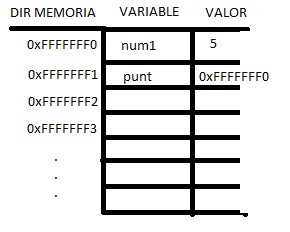
\includegraphics[width=0.4\textwidth]{resources/puntero.jpg}
        \caption{Ejemplo de puntero \textit{punt} que referenciua a la dirección de 
        memoria \textit{0xFFFFFFF0} que es, a su vez, la variable entera \textit{num1}
        que almacena el valor \textit{5}.}
        \label{puntero}
    \end{figure}

    Los punteros pueden apuntar a variables previamente declaradas o a variables dinámicas.

    \begin{quote}
        \small \textit{La potencia de los punteros reside en poder crear (reservar memoria) y 
        destruir (liberar memoria) una variable (dinámica) en tiempo de ejecución.}
    \end{quote}

    Un puntero ocupa normalmente 4 bytes y se declara siempre de acuerdo con el tipo de dato al que apunta.

    \begin{lstlisting}[language=C,numbers=left]
    // La declaracion de punteros en C se realiza 
    // anteponiendo (*) al nombre de la variable.
    int * x;\end{lstlisting}

    \subsection{Operadores de dirección e indirección}

    El lenguaje C dispone de los operadores de \textbf{dirección} (\textit{$\&$}) e \textbf{indirección} 
    (\textit{$*$}) permitiendo respectivamenta acceder a la dirección asociada a una determinada variable
    y acceder al contenido de ésta (zona de memoria) a la que apunta el puntero.

    \begin{lstlisting}[language=C,numbers=left]
    // Variables estaticas 'i' y 'j', puntero 'p'. 
    int i, j, *p;
    // El puntero 'p' apunta a 'i'; asignamos a la 
    // variable 'p' la direccion de memoria de la 
    // variable 'i'.
    p = &i;
    // Asignamos a la direccion de memoria a la que 
    // apunta 'p' el valor '10'.
    *p = 10;
    // Cambiamos el puntero a la variable 'j' y le 
    // asignamos dinamicamente un valor a esta.
    p = &j;
    *p = -2;
    // Cambiamos el puntero de nuevo para que no 
    // apunte a ninguna variable.
    p = NULL;\end{lstlisting}

    Podemos trabajar con punteros de tipo indefinido con \textit{$void *$}, pudiendo asignarse cualquier
    tipo de puntero y valor; es un puntero genérico a alguna parte donde se almacena información
    de algún tipo. Es el programador el responsable de definir estos <<algún>> eliminando esta 
    ambigüedad.

    \begin{lstlisting}[language=C,numbers=left]
    int x = 1;
    float r = 1.0;

    void* ptr = &x;
    *(int *)ptr = 2;

    ptr = &r;
    *(float *) ptr = 1.1;\end{lstlisting}

    \subsection{Aritmética de punteros}

    Las operaciones aritméticas entre punteros en el lenguaje C se limitan a \textbf{suma}, 
    \textbf{resta}, \textbf{comparación} y \textbf{asignación}.

    Las operaciones aritméticas en los punteros a un tipo de dato $x$ tienen automáticamente en 
    cuenta el tamaño que ocupa ese tipo de dato en memoria. Es decir, el número de \textit{bytes}
    necesario para almacenar un objeto de ese tipo de dato: la suma incrementa la dirección a 
    la que apunta el puntero teniendo en cuenta el tipo de dato que al que apunta el puntero (si 
    un puntero apunta a un tipo de dato entero y se le suma 1, se desplaza el tamaño de un entero).
    En el caso de la resta, se decrementa la dirección.

    Estas dos operaciones son útiles cuando trabajamos con vectores o matrices (lineal) y la suma
    o resta permitirían moverse entre los elementos de éste.

    \begin{lstlisting}[language=C,numbers=left]
    int a, b, c;
    int *p1, *p2;
    void *p;

    p1 = &a;
    *p1 = 1;

    p2 = &b;
    *p2 = 2;

    p1 = p2;
    *p1 = 0;

    p2 = &c;
    *p2 = 3;

    p = &p1;
    *p = p2;
    *p1 = 1;\end{lstlisting}

    \subsection{Vectores, matrices y punteros}

    Un vector es un puntero al primer elemento del propio vector, contiene la dirección donde
    se encuentra el primer elemento. Es un puntero constante y no puede modificarse su 
    contenido, siendo la dirección que contiene a la que apunta.

\section{Ficheros}

    Los datos en memoria son siempre volátiles, pero a menudo tendremos la necesidad de que nuestros 
    datos permanezcan; lo que se puede conseguir almacenándolos en un soporte físico. De tal forma que 
    puedan ser recuperados tras finalizar el programa o apagar el equipo. Esto puede conseguirse 
    fácilmente con los \textbf{ficheros}.

    Un fichero es un conjunto de datos estructurado en una colección de entidades elementales denominadas 
    \textbf{registros}. Estos registros son por norma general de igual tipo y constan a su vez de diferentes entidades 
    de nivel más bajo, llamadas \textbf{campos}. Un conjunto de ficheros relacionados se conoce con el nombre 
    de \textbf{base de datos}.

    \subsection{El buffer}

        Hasta ahora la metodología de trabajo del código puede expresarse de forma sencilla bajo el 
        esquema $CPU\iff MEMORY$. Pero añadiendo la capacidad de acceso a disco (ficheros), quedaría 
        un esquema $CPU\iff MEMORY\iff HD$.

        Es imposible pasar datos directamente desde la CPU al HD (disco). Los soportes externos a su vez 
        son extremadamente lentos si los comparamos a las velocidades de la CPU. Si esta comunicación 
        fuera hipotéticamente directa, para que fuese eficaz debería seguir el ritmo del dispositivo lento,
        lo que implicaría un total desaprovechamiento de la velocidad de procesamiento de nuestra máquina.

        Para paliar esta deficiencia nos serviremos de lo que se denomina como \textbf{buffer}, que es 
        una memoria intermedia. Dejando un esquema $CPU\iff MEMORY\iff Buffer\iff HD$. Así el buffer 
        supone un elemento mediador y regulador que siempre se interpone entre la memoria y el dispositivo 
        físico.

        Este buffer puede localizarse tanto en la controladora del dispositivo como en la caché de la placa; 
        siendo pocos los lenguajes de programación que permiten la manipulación directa de datos en el 
        buffer. En este selecto grupo se encuentra C.

    \subsection{Transferencia entre registros físicos y lógicos}

        El término \textbf{registro} está ligado directamente al trabajo con el buffer. Al dimensionar 
        el buffer aparecen nuevos conceptos de registro:

        El registro lógico es la estructura de datos que el programador se ha definido. Mientras que 
        el registro físico es la estructura de datos mínima que se va a transferir en una 
        operación E/S.

        Al realizar pues operaciones de entrada/salida nos encontramos en diferentes situaciones en 
        relación a ambas naturalezas de los registros.

        \subsubsection{Tamaño de registro lógico superior al tamaño de registro físico $l>f$}

            Pongámonos en una situación de operación de lectura de un texto al que:

            Con un tamaño lógico de 100 bytes y un tamaño físico de 20 bytes se verá obligado a realizar
            5 operaciones de lectura ($5\times 20$) para conseguir presentarnos los 100 bytes.

            Obviamente es un sistema lento, lentitud que se agrava seriamente si lo implementamos en 
            una red; hasta tal punto que podría saturarse hasta caerse, si hubiera muchos accesos 
            concurrentes.\footnote{
                Este sistema está anticuado, solía estar presente en sistemas monotarea. También se 
                observa en tareas de mantenimiento.
            }

        \subsubsection{Tamaño de registro lógico igual a tamaño de registro físico $l = f$}

            En esta situación la actuación es sencilla, siendo $x$ peticiones $\rightarrow$ $x$
            operaciones E/S.

            Es el caso ideal para operaciones de actualización, aún así no es el tipo ideal para 
            todo tipo de operaciones, entre ellas las operaciones de tipo consulta, que se puede 
            mejorar con otro tipo de gestión del buffer como veremos más adelante.

        \subsubsection{Tamaño de registro lógico menor que tamaño de registro físico $l<f$}

            Nos encontramos en el caso en que pedimos una unidad y el dispositivo nos devuelve una cantidad 
            superior. Por ejemplo, pedimos 1 byte y recibimos 5 bytes.

            Esta gestión presenta varios problemas:

            \begin{itemize}
                \item Mayor consumo de memoria.
                \item Hasta que no se tienen los $x$ procesados el sistema no graba; y si ocurriera algún 
                problema se perderían datos. 
                \item <<\textbf{Bloqueo}>>. Se produce cuando un usuario pide 1 registro y se le conceden 5 
                por defecto. Estos 5 quedarán bloqueados y no podrá acceder nadie a ellos hasta que sean liberados
                por quien los solicitó primero.\footnote{
                    Existen lenguajes como Cobol que pueden parametrizar este bloqueo ()\textit{Facotr de bloqueo}).
                }
            \end{itemize}

            Como bien indicamos anteriormente, para realizar consultas este es el caso más óptimo. Sin embargo
            su eficacia es muy pobre para realizar mantenimientos a causa de los registros que permanecen 
            bloqueados, y que quizás contengan datos que ni siquiera serán procesados.

    \subsection{Tipos de ficheros}

        Los ficheros pueden ser clasificados de innumerables maneras, pero en este caso nos interesa 
        una única clasificación, que se hace en función del acceso a los mismos.

        \subsubsection{Ficheros secuenciales}

            En los ficheros secuenciales un registro se encuentra a continuación de otro, por lo que 
            para poder leer el registro $n$ se deberán leer también los $n-1$ anteriores ($R_1, R_2,R_3...R_n$).

            La ubicación física de este tipo de ficheros puede ser cualquier dispositivo.

            \paragraph{Inconvenientes} El mayor inconveniente de este tipo de archivos es la lectura, ya que 
            para leer el registro 1.000 se deberán leer los 999 anteriores. No poseen registros clave ni 
            identificadores, tampoco se encuentran ordenados. Son una única pila de datos.

        \subsubsection{Ficheros de acceso directo}

            En los ficheros de acceso directo cada registro ocupa una posición física que le corresponde, 
            por lo que dentro de cada registro deberá existir un campo clave.
            Dicho campo clave almacenará la dirección física donde se almacenan los datos, siendo el 
            99\% de las ocasiones un campo de tipo numérico.

            En los ficheros de acceso directo se puede acceder a $R_n$ sin necesidad de pasar por los 
            $n-1$ anteriores.

            Este modelo no siempre es la solución ideal, pues en ocasiones se puede infrautilizar el espacio
            de disco. Siendo el factor de rentabilidad que recomienda el uso de los ficheros de acceso directo 
            una tasa de ocupación del 75\% en adelante.

            \paragraph{Inconvenientes} La clave es una gran ventaja y, a su vez, un inconveniente debido a la 
            necesidad imperante de conocer la clave. Otro inconveniente es la necesidad de estar en un soporte 
            de datos tales como CD, HD... No será posible su aplicación en almacenamiento sobre soportes 
            secuenciales como cintasmagnéticas.

        \subsubsection{Ficheros indexados}

            La mayoría de los lenguajes proporcionan el soporte para los dos tipos de ficheros anteriores.
            En cambio, el soporte para ficheros indexados lo aportan muy pocos lenguajes\footnote{
                COBOL es uno de los pocos lenguajes que implementan de forma nativa el soporte y tratamiento 
                de ficheros indexados.

                C no aporta las funcionalidades necesarias para ello. No obstante si que podemos encontrar
                algunas librerías de terceros que las implementan.
            }.

            Los ficheros indexados se caracterizan por un almacenamiento secuencial de los datos (capacidad 
            óptima) y un acceso directo a la información (valocidad\footnote{
                La velocidad de un fichero indexado no es tan alta como la de un fichero de acceso directo, ya 
                que un indexado siempre recorre índices. 

                No obstante sus velocidades medias son considerablemente elevadas.
            }).

            Este tipo de ficheros permite el uso de claves alfanuméricas, creando el concepto de \textbf{clave 
            alternativa} mediante las cuales se consigue realizar búsquedas ordenadas según varios campos.

            \paragraph{Estructura de un fichero indexado}

            Lo primero que contiene un fichero indexado son los datos, siendo la totalidad de los registros 
            grabados \textbf{secuencialmente}.

            Por otro lado necesitamos velocidad de acceso, por lo que existe otro fichero denominado 
            \textbf{fichero de índices}\footnote{
                Un fichero de índices es también de estructura secuencial.
            }, que almacena precisamente la sencuencia de índices (también almacenado
            en el fichero de datos).

            Cada uno de estos elementos se corrsponde con una dirección física que apunta al fichero de los datos 
            y el campo clave definido por el programador.

            \begin{figure}[htp]
                \centering
                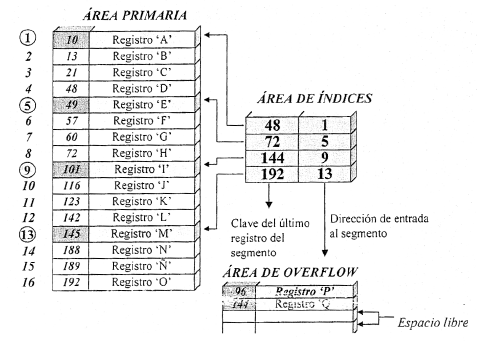
\includegraphics[width=0.6\textwidth]{resources/ficheros01.png}
                \caption{Representación gráfica de un fichero indexado.}
                \label{ficheros01}
            \end{figure}

            El fichero de índices está siempre ordenado según la clave, ya sea ascendiente o descendientemente.
    
    \subsection{Flujos de datos}

        El concepto de flujo es un concepto abstracto representativo de una operación de movimiento 
        de datos desde un origen hasta un destino. Conceptualmente, entre ambos (origen y destino) se establece
        lo que se denomina un \textbf{canal}, que es por donde circulan los datos. Este término de canal, 
        debido a la herencia UNIX también suele denominarse como \textbf{pipe}.

        En las ciencias informáticas, a menudo encontraremos referencia a flujos usando su equivalente 
        anglosajón: \textbf{stream}.

        \subsubsection{Flujos estándares en C}

            El lenguaje C ofrece 3 flujos abiertos y dispuestos para su utilización directa, herencia 
            directa de UNIX:

            \paragraph{stdin} Se asocia direcamente a la entrada estándar, siendo el teclado.
            \textit{scanf} trabaja implícitamente con \textbf{stdin}.

            \begin{lstlisting}[language=C,numbers=left]
    extern FILE *stdin; \end{lstlisting}
            
            \paragraph{stdout} Se asocia directamente a la salida estándar, siendo la pantalla. 
            \textit{printf} trabaja implícitamente con \textbf{stdout}.

            \begin{lstlisting}[language=C,numbers=left]
    extern FILE *stdout; \end{lstlisting}
        

            \paragraph{stderr} Está vinculada a la salida estándar de errores, y al igual que 
            \textbf{stdout} es la pantalla. 

            \begin{lstlisting}[language=C,numbers=left]
    extern FILE *stderr; \end{lstlisting}
        
            El trabajo con archivos en C está directamente intervenido por un buffer. Así, se permite trabajar
            con secuencias de datos independientemente de la naturaleza de las mismas, pudiendo trabajar 
            siempre de una forma estandarizada y cómoda.

    \subsection{Punteros a fichero \textit{FILE*}}

        C establece en su librería estándar (\textit{stdio.h}) una estructura específica para el manejo 
        de datos. Ésta permite manejar archivos mediante un nombre lógico para su fácil identificación.
        Además, almacena información relativa a la dirección del buffer que se encarga de su manejo, el 
        control de caracteres, tipo de apertura, etc.

        La estructura definida \textit{FILE} se implementa de la siguiente forma:

        \begin{lstlisting}[language=C,numbers=left]
    typedef struct{
        short level;
        unsigned flags;
        char fd;
        unsigned char hold;
        short bsize;
        unsigned char *buffer, *curp;
        unsigned istemp;
        short token;
    } FILE; \end{lstlisting}
    

    \subsection{Manejo de ficheros y operaciones sobre éstos}

        \subsubsection{Apertura de ficheros}

            Es lógicamente la primera operación que debemos realizar con un fichero antes de poder 
            trabajar con él, de forma que conectemos un fichero físico con nuestra representación lógica 
            de dicho fichero, es decir, con un FILE *.

            Para ello se utiliza la función \textit{fopen}, cuyo prototipo es el siguiente:

            \begin{lstlisting}[language=C,numbers=left,basicstyle=\small]
    FILE *fopen(const char *nombre_fichero, const char *modo);\end{lstlisting}

            A esta función se de le deben pasar como argumentos el nombre del fichero físico (con su ruta)
            y el modo de apertura que deseamos\footnote{
                Estos modos de apertura pueden ser:

                \begin{itemize}
                    \item \textbf{r}. Apertura de lectura.
                    \item \textbf{w}. Apertura de escritura, si el fichero ya existe lo crea nuevo vacío,
                    perdiendo todos los datos que pudieran existir.
                    \item \textbf{a}. Apertura para escritura al final del fichero, añadiendo datos. Escribe 
                    a partir de la marca anterior de fin de fichero.
                    \item \textbf{r+}. Apertura de actualización (lectura/escritura). Es requisito imprescindible
                    que el fichero exista previamente.
                    \item \textbf{w+}. Apertura para actualización (lectura/escritura). A diferencia que \textbf{r+},
                    si el fichero no existe lo creará; y si este existe lo sobrescribirá por uno nuevo vacío.
                    \item \textbf{a+}. Apertura para actualización al final del archivo (lectura/escritura). Si el 
                    fichero no existe lo creará.
                \end{itemize}

                Además, en Cdistinguimos entre 2 tipos de o clases de ficheros ateniendo 
                a la naturaleza de sus datos:

                \begin{enumerate}
                    \item \textbf{Fichero de texto}, que permite el almacenamiento de caracteres (concretamente 
                    su código ASCII). Cabe destacar que para almacenar información numérica en un archivo de texto 
                    es necesario convetirla previamente a caracteres.
                    \item \textbf{Fichero binario}, que almacenan información binaria.
                \end{enumerate}

                Para indicar a que tipo de fichero queremos acceder indicaremos en el modo de apertura una $t$ o 
                una $b$, para indicar si es un fichero de texto o binario, respectivamente. Por lo tanto, tendremos
                los siguientes modos de apertura válidos:

                \[rt, rb, wt, wb, at, ab r+t, r+b, w+t, w+b, a+t, a+b\]
            }.

            La función finalmente nos devolverá un FILE * que cntendrá la dirección a una estructura FILE 
            que nos permitirá referenciar al fichero. 

        \subsubsection{Macros}

            Cuando se trabajan con ficheros hay un par de macros incluidas en \textit{stdio.h} que son muy 
            utilizadas:

            \paragraph{Macro NULL} FILE * es un puntero, y como tal se usa para comprobar si dicho puntero 
            almacena una dirección de memoria válida o no apunta a nada.

            \paragraph{Macro EOF} Este macro se utiliza para detectar el final de fichero. Su origen está 
            en la función \textit{feof}, cuyo prototipo es:

            \begin{lstlisting}[language=C,numbers=left]
    int feof (FILE *stream);\end{lstlisting}

            Esta función devuelve un valor distinto a 0 si no se alcanzó la marca de fin de fichero.

        \subsubsection{Cierre de ficheros}

            Como es lógico, es más que recomendable cerrar los ficheros que no se van a utilizar. También 
            cerrarlos si momentáneamente no van a ser accedidos (evitando problemas de concurrencia).

            Este hecho de cerrar los ficheros es más important cuando tratamos con operaciones de 
            escritura, ya que el hecho de cerrar un fichero implica llevar el contenido del buffer al 
            dispositivo físico (podríamos decir que guardamos el contenido). De no hacerse esta acción, 
            podría ocasionar en la pérdida de los datos en el buffer.

            No obstante los sistemas operativos cierran los ficheros cuando se destruyen sus descriptores, 
            de forma que no se produzcan inconsitencias de datos.

            Para cerrar los ficheros se utiliza la función \textit{fclose}, cuyo prototipo es:

            \begin{lstlisting}[language=C,numbers=left]
    int fclose (FILE *puntero_fichero);\end{lstlisting}
        
        \subsubsection{Lectura y escritura de carácter}

            Para ello haremos uso de \textit{fgetc}, cuyo prototipo es:

            \begin{lstlisting}[language=C,numbers=left]
    int fgetc (FILE *flujo);\end{lstlisting}

            Lee el siguiente carácter de un FILE * y devuelve el valor en forma de entero.
            Cuando se produce un error o se alcanza la marca de fin de fichero se devuelve
            EOF. 

            La escritura de carcacteres se realiza con la función \textit{fputc}, 
            cuyo prototipo es:

            \begin{lstlisting}[language=C,numbers=left]
    int fputc (int caracter, FILE *flujo);\end{lstlisting}
        
            Al que le pasamos como parámetro el carácter que deseamos escribir en 
            modo numérico y la dirección del flujo destino. Si la operación se realizó
            con éxito se devuelve el propio carácter, si no, se devuelve EOF.

        \subsubsection{Lectura y escritura de cadenas}

            La lectura de cadenas\footnote{
                Recuerde: las cadenas como tal no existen en el lenguaje C, cuando se 
                habla de cadenas nos referimos al concepto detrás de las secuencias 
                de caracteres (char); char[].
            } de caracteres desde el archivo asociado se recupera 
            a través de la función \textit{fgets}, cuyo prototipo es:
            
            \begin{lstlisting}[language=C,numbers=left]
    char *fgets (char *cadena, int n, FILE *flujo);\end{lstlisting}
        
            La recuperación de la cadena se lleva a cabo hasta que es leído el carácter 
            de fin de línea ($\backslash n$) o bien hasta alcanzar el valor de 
            $n-1$ caracteres leídos; siendo $n$ el argumento que se le pasa a la función.
            Si la operación concluye con éxito, devuelve un puntero a la cadena recuperada;
            en caso contrario devuelve $NULL$.

            La escritura de cadenas en un flujo se realiza mediante la función \textit{fputs},
            cuyo prototipo es:

            \begin{lstlisting}[language=C,numbers=left]
    int fputs (const char *cadena, FILE *flujo);\end{lstlisting}
        
            Pasándole la dirección de la cadena y la dirección al propio flujo. Si la 
            cadena acaba en $\backslash 0$ la copia como tal; en caso contrario 
            añade un salto de línea ($\backslash n$) y la copia sin la marca de fin $\backslash 0$.
            Si la operaciñón concluye con éxito devuelve un valor numérico positivo; en caso 
            contrario devuelve EOF.

        \subsubsection{Lectura y escritura de datos binarios}\label{ficherosbinarios}

            La función para la lectura de estructuras binarias es \textit{fread}, 
            y lee de un archivo de $n$ bloques de bytes y los deja en un buffer 
            específico apuntado por un puntero sin tipo. El prototipo es:
            
            \begin{lstlisting}[language=C,numbers=left]
    size_t fread (void *ptr, size_t t, size_t n, FILE *flujo);\end{lstlisting}

            Recibiendo como parámetros:

            \begin{itemize}
                \item Un puntero sin tipo que referenciará a la estructura donde se almacenan los 
                datos leídos.
                \item El tamaño de elemento que va a ser leído.
                \item El número de elementos que serán leídos.
                \item Un puntero de tipo fichero que referencia al fichero donde están almacenados 
                los datos, siendo el origen del flujo.
            \end{itemize}

            La función para la escritura de estructuras binarias es \textit{fwrite}, 
            cuyo prototipo responde a la siguiente firma:
            
            \begin{lstlisting}[language=C,numbers=left,basicstyle=\small]
    size_t fwrite (const void *ptr, size_t size, size_t n, FILE *flujo);\end{lstlisting}
        
            Recibiendo como parámetros:

            \begin{itemize}
                \item Un puntero sin que referenciará a la estructura que contiene la dirección 
                de los datos que van a ser escritos.
                \item El tamaño del elemento que va a ser escrito.
                \item El número de elementos de este tipo que se escribirán.
                \item Un puntero de tipo fichero, que referencia al flujo donde se escribirán los datos, 
                es decir, el destino del flujo.
            \end{itemize}

            La función devuelve el número de elementos que realmente fueron escritos.

        \subsubsection{Funciones para ficheros de acceso directo}

            Normalmente cuando se quiere trabajar en C con ficheros de acceso directo 
            se usan ficheros binarios (véase apartado \ref{ficherosbinarios}).

            Las funciones de \textit{stdio.h} más utilizados para éste propósito son:

            \paragraph{Rebobinado} La función se denomina \textbf{rewind}. No es 
            exclusiva para los ficheros de acceso directo, aunque debido a su modo de 
            operación se incluye en esta categoría. 

            Mediante rewind situamos el puntero del flujo referenciado al comienzo 
            del mismo, siendo su prototipo:

            \begin{lstlisting}[language=C,numbers=left]
    void rewind (FILE *flujo);\end{lstlisting}

            \paragraph{Posicionamiento} Los ficheros de acceso directo permiten 
            situarse en una posición puntual a lo largo del fichero. La función 
            que realiza esta acción se denomina \textbf{fseek}. Su prototipo es:

            \begin{lstlisting}[language=C,numbers=left,basicstyle=\small]
    int fseek (FILE *flujo, long desplazamiento, int referencia);\end{lstlisting}
        
            Recibiendo los siguientes parámetros:

            \begin{itemize}
                \item Flujo objeto del desplazamiento.
                \item Cantidad de bytes desplazados, expresados en un valor numérico 
                de tipo long.
                \item Referencia de desplazamiento\footnote{
                    Para referenciar el desplazamiento \textit{stdio.h} nos ofrece 3
                    constantes en forma de macros:

                    \begin{enumerate}
                        \item \textbf{SEEK\_SET}, cuyo valor se corresponde con 0, referenciando 
                        al inicio del flujo.
                        \item \textbf{SEEK\_CUR}, cuyo valor se corresponde con 1, referenciando 
                        la posición actual.
                        \item \textbf{SEEK\_END}, cuyo valor se corresponde con 2, referenciando 
                        la posición final.
                    \end{enumerate}
                }, desde donde partiremos.
            \end{itemize}

            Además, \textit{stdio.h} nos brinda otra función complementaria denominada 
            \textit{ftell}, usada para consultar la posición actual del puntero expresada 
            como el número de bytes desplazados desde el incicio del flujo. Respondiendo 
            al siguiente prototipo:
            
            \begin{lstlisting}[language=C,numbers=left,basicstyle=\small]
    long int ftell (FILE *flujo);\end{lstlisting}

            En caso de error devuelve $-1L$.
        
\section{Listas enlazadas}\label{listasenlazadas}

    Una lista enlazada es una colección de elementos homogéneos llamados nodos con una relación
    lineal entre ellos ($a_i$ sucede a $a_{i-1}$) y cumple con las siguientes características:
    
    \begin{itemize}
        \item Cada nodo, exceptuando el primero, tiene un predecesor; así como cada nodo, 
        exceptuando el último, tiene un sucesor.
        \item Es una estructura de datos dinámica (véase sección \ref{estructuradinamica}). Es 
        decir, cada uno de sus nodos puede aumentar o disminuir en tiempos de ejecición.
        \item Todos sus elementos son accesibles.
        \item Pueden insertarse y/o eliminarse nodos en cualquier posición de la lista.
    \end{itemize}

    Por lo que podemos definir una lista enlazada como:

    \begin{quotation}
        \small <<Es una estructura de datos dinámica cuyos nodos están referenciados 
        unos a otros linealmente, de forma que el nodo anterior referencia a su 
        siguiente (a excepción del último).>> (véase figura \ref{listaenlazada01})
    \end{quotation}

    \begin{figure}[htp]
        \centering
        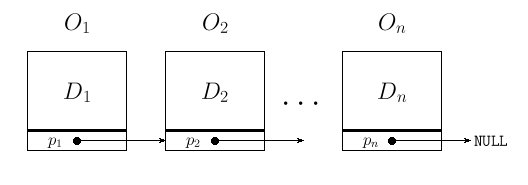
\includegraphics[width=0.4\textwidth]{resources/listaenlazada01.jpg}
        \caption{Definición gráfica de lista simplemente enlazada.}
        \label{listaenlazada01}
    \end{figure}

    \subsection{Implementación de listas enlazadas estáticas}

        La implementación de una lista enlazada puede hacerse de dos formas; el primero de 
        ellos basado en estructuras estáticas (\textit{arrays}) que recibe el nombre de 
        \textbf{listas estáticas} y el segundo basado en estructuras dinámicas (
        \textit{memoria dinámica}) que se conoce como \textbf{listas enlazadas}.

        La implementación de las \textbf{listas estáticas} es sencillo:

        \begin{lstlisting}[language=C,numbers=left]
    Struct Lista {
        // TipoDato Elementos [N];
        int Numeros [10];
        // int UltimoElemento;
        int ultimoNumero; // Numero entero que indica la 
        // posicion en la que se encuentra el ultimo elemento
        // de la lista, dentro del array.
    };\end{lstlisting}

        Nos centraremos en el segundo modo de implementación, que es el más comúnmente 
        utilizado y el que mejor gestión hace de los recursos de memoria.

    \subsection{Clasificaciones de las listas enlazadas}
        
        \subsubsection{Según el número de enlaces entre nodos}

            \paragraph{Listas simplemente enlazadas} Es un conjunto de nodos conectados 
            entre si por un único enlace, de tal forma que el enlace de dicho elemento de
            la lista nos permite acceder al inmediatamente siguiente, si éste existiera. 
            (véase figura \ref{listaenlazada01}). Son óptimas para recorridos hacia delante. 

            \paragraph{Listas doblemente enlazadas} \label{listadoblementeenlazada} 
            El concepto mismo de lista doblemente enlazada es una extensión basada en la lista simplemente 
            enlazada (véase apartado \ref{listasenlazadas}). Pero a diferencia de las listas simplemente enlazadas, 
            que sólo pueden recorrerse en un único sentido, concretamente hacia delante, las listas doblemente 
            enlazadas permiten recorrer la lista enlazada en ambos sentidos, tanto adelante como hacia 
            atrás. Recuerde la figura \ref{listaenlazada02}.
    
            En éstas, cada nodo de la lista se encuentra enlazado tanto con el siguiente como con el anterior.
    
            \begin{lstlisting}[language=C,numbers=left]
            struct Nodo 
            {
                Dato d;
                struct Nodo *siguiente;
                struct Nodo *anterior;
            };\end{lstlisting}
    
            El acceso a la lista se realizará también de manera idéntica a como lo hacíamos con las listas 
            con enlace simple, mediante un puntero que referenciase a la cabeza.
    
            \begin{lstlisting}[language=C,numbers=left]
            int main() {
                Nodo *cabeza = NULL;
            }\end{lstlisting}
    
    
            
            \begin{figure}[htp]
                \centering
                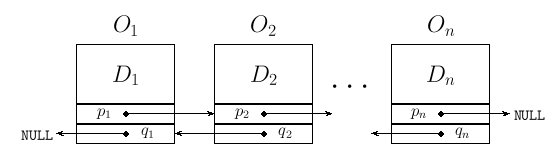
\includegraphics[width=0.6\textwidth]{resources/listaenlazada02.jpg}
                \caption{Definición gráfica de lista doblemente enlazada.}
                \label{listaenlazada02}
            \end{figure}        

        \subsubsection{Según linealidad}

            \paragraph{Listas lineales} Son aquellas cuya única forma de recorrerlas es en
            línea recta. Es decir, cuando estamos situados al inicio debemos avanzar obligatoriamente
            a su elemento siguiente; y cuando estamos en el final debemos retroceder al elemento 
            anterior, siempre que se trate de una lista \textit{doblemente enlazada}.
        
            \paragraph{Listas circulares} Son una especialización de las listas lineales en 
            las que el último nodo tiene como nodo inmediatamente posterior el que encabeza
            la lista (véase figura \ref{listaenlazada02circular}).

            \begin{figure}[htp]
                \centering
                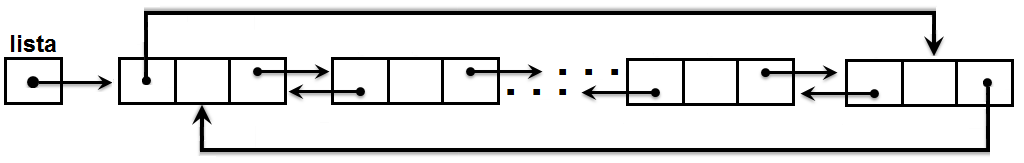
\includegraphics[width=0.6\textwidth]{resources/listaenlazada02.png}
                \caption{Definición gráfica de lista doblemente enlazada circular.}
                \label{listaenlazada02circular}
            \end{figure}    

            Las listas circulares son listas enlazadas, sean mediante enlace simple o enlace doble, pero 
            con la peculiaridad de que el último elemento apunta al primero (y no a $NULL$). Cabe destacar 
            que si la lista circular es además doblemente enlazada, el puntero anterior del primer elemento 
            deberá también apuntar al último nodo.
    
            Este tipo de listas no tiene conceptualmente un principio ni un final predefinidos, no obstante
            para acceder a ella necesitaremos un puntero a un nodo que nos facilite el acceso a la misma.
    
            El principal problema que nos presenta este tipo de líneas es la posibilidad de caer en un 
            bucle infinito al recorrerlas, puesto que no hay un final definido. Para evitarlo, almacenamos 
            la referencia (en forma de puntero, lógicamente) del último elemento insertado, de modo que 
            consideramos éste como el final ficticio de la lista sin final. Por lógica, el principio 
            ficticio será el siguiente a éste.    

    \subsection{Componentes de la lista enlazada}

        \subsubsection{Nodos}

            Ya conocemos de qué se trata un nodo, cada uno de los elementos que conforman 
            la lista. Estos tienen la siguiente estructura normalmente:

            \begin{lstlisting}[language=C,numbers=left]
    struct nodo {
        // TipoDato dato;
        int id;
        struct nodo* pSig; // Referencia a uno o mas
        // nodos de la lista que vayamos a crear. 
        // Gracias a ella podremos pasar de un nodo 
        // a otro. Estas referencias se implementan 
        // mediante punteros.
    };\end{lstlisting}

            Resumiendo, un nodo de una lista se divide en \textit{información} y \textit{enlaces}.

        \subsubsection{Punteros de acceso}

            El hecho de que los elementos de la lista se encuentren enlazados, permite acceder
            desde un elemento a todos sus posteriores (y anteriores si se trata de una lista 
            doblemente enlazada, véase \ref{listadoblementeenlazada}) siguiendo los punteros que 
            los enlazan. Necesitamos pues almacenar siempre la dirección del primer nodo de la 
            lista, a través del cual accedemos a ella, siendo nuestra puerta a la lista.

            Esta referencia al principio de la lista será un puntero que almacenará la dirección 
            del primer nodo de la lista, siempre y cuando la lista no esté vacía. A este puntero se 
            le denomina \textit{cabeza de la lista}, \textit{puntero de la cabeza}, \textit{puntero inicio}\dots
            (véase figura \ref{listaenlazada03})

            \begin{figure}[htp]
                \centering
                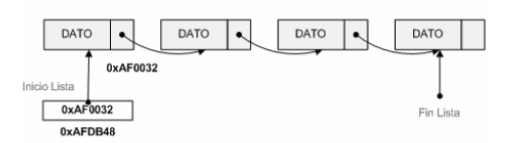
\includegraphics[width=0.6\textwidth]{resources/listaenlazada03.png}
                \caption{Puntero a la cabeza en lista simplemente enlazada.}
                \label{listaenlazada03}
            \end{figure}

            También es recomendable crear un acceso al último nodo de la lista (aquel que no tiene elemento 
            siguiente), ya que algunas operaciones trabajan directamente con este último nodo.
            (véase figura \ref{listaenlazada04})

            \begin{figure}[htp]
                \centering
                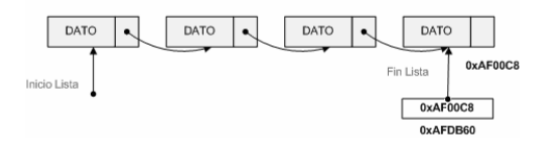
\includegraphics[width=0.6\textwidth]{resources/listaenlazada04.png}
                \caption{Puntero al final de la lista simplemente enlazada.}
                \label{listaenlazada04}
            \end{figure}
                
    \subsection{Operaciones con listas enlazadas}

        \subsubsection{Creación de lista enlazada} 
        
            La creación de la lista consiste básicamente en declarar la estructura que ésta 
            tendrá, es decir, los elementos que la compondrán y el puntero que apuntará al 
            primer elemento de la misma\footnote{
                Cabe destacar que puede crearse una lista vacía, sin ningún elemento, para 
                ir insertándolos posteriormente mediante la operación de inserción (véase 
                \ref{listaenlazada_insercion})
            }.

            Para llevar a cabo la creación de la lista es necesario primero declarar el tipo 
            de elemento que contendrá, así como una referencia (puntero) al que será el primero.
            En caso de una lista vacía inicialmente, no será necesario crear ningún nodo, simplemente
            el puntero al inicio apuntará a \textit{NULL}.

            \begin{lstlisting}[language=C,numbers=left]
    Struct Coordenada {
        float ejeX;
        float ejeY;
        float ejeZ;
    };

    void main() {
        struct Nodo * pPrimero = NULL;

        // [...]
    }\end{lstlisting}

            Si por el contrario la lista será creada con algún nodo, habrá que reservar memoria
            para él. Para ello realizaremos una llamada a alguna de las funciones que permiten hacerlo 
            (\textit{malloc}, \textit{calloc} ó \textit{realloc}, véase TODO) y almacenaremos
            el puntero que nos devuelven estas funciones, previo \textit{casting}.
            
            \begin{lstlisting}[language=C,numbers=left]
    Nodo * pNodo = (Nodo *) malloc (sizeof(Nodo));\end{lstlisting}

            \begin{enumerate}
                \item Si el nodo que creamos es el primer nodo de la lista utilizaremos el puntero 
                a la cabeza de la lista.
                \item Si por el contrario el nodo no es el primero, utilizaremos el puntero del 
                último elemento de la lista.
            \end{enumerate}

        \subsubsection{Calcular la longitud de una lista enlazada}

            Para calcular el número de elementos de una lista, el algoritmo no puede ser más
            simple. Inicializamos un contador a cero y, recorremos la lista hasta el final.
            Con cada iteración, aumentamos en uno el contador. De forma que al finalizar el bucle
            el contador tendrá almacenado el número de elemetnos que componen la lista.

            Para facilitar su uso se ha centralizado en una función denominada \textit{longitudl}.
            
        \begin{lstlisting}[language=C,numbers=left]
    int longitudl(struct lista *l) {
        struct lista *p;
        int n;
        n = 0;
        p = l;
        while (p != NULL) {
            ++n;
            p = p->sig;
        }
        return n;
    }\end{lstlisting}

        \subsubsection{Inserción de elementos en lista enlazada}\label{listaenlazada_insercion}

            \paragraph{Inserción al comienzo de la lista} Sea $x$ una estructura tipo dato 
            y $l = (O1, O2, ... , On)$ una lista, esperando el resultado $(x, O1, O2, ... , On)$.
            Para ello creamos un nuevo nodo, siendo en concreto una llamada \textit{malloc}. Para 
            facilitar el desarrollo lo haremos en una función (véase figura \ref{listaenlazada05}).

            \begin{lstlisting}[language=C,numbers=left]
    struct lista *crearNodo(void) {
        return (struct lista *) malloc(sizeof(struct lista));
    }\end{lstlisting}

            \begin{figure}[htp]
                \centering
                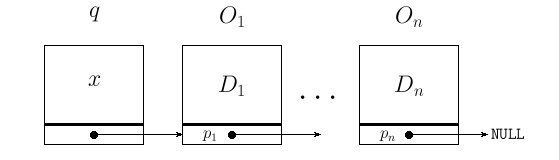
\includegraphics[width=0.6\textwidth]{resources/listaenlazada05.jpg}
                \caption{Diagrama de creación de elemento al comienzo de la lista enlazada.}
                \label{listaenlazada05}
            \end{figure}

            Posteriormente será necesario crear una función que nos facilite la llamada, recibiendo
            como parámetro la propia lista y el elemento estructura que, que es el nodo.

            \begin{lstlisting}[language=C,numbers=left]
    struct lista *insertComienzo(struct lista *l, struct dato x) {
        struct lista *q;
        q = crearNodo(); 
        q->datos = x; 
        q->sig = l;
        l = q;
        return l;    
    }\end{lstlisting} 
            
            \paragraph{Inserción al final de la lista} Sea $x$ una estructura tipo dato 
            y $l = (O1, O2, ... , On)$ una lista, esperando el resultado $(O1, O2, ... , On, x)$
            (véase figura \ref{listaenlazada06}).

            \begin{figure}[htp]
                \centering
                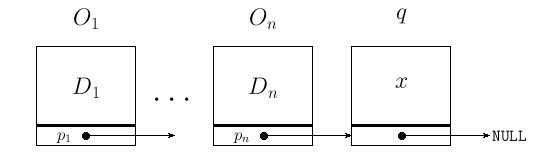
\includegraphics[width=0.6\textwidth]{resources/listaenlazada06.jpg}
                \caption{Diagrama de creación de elemento al final de la lista enlazada.}
                \label{listaenlazada06}
            \end{figure}

            La función de inserción al final tiene dos posibles caminos: si la lista está vacía 
            (\textit{NULL}) el resultado será $l = (x)$. En caso de no estar vacía situaremos el puntero 
            en el último elemento.

            \begin{lstlisting}[language=C,numbers=left]
    struct lista *insertFinal(struct lista *l, struct dato x) {
        struct lista *p,*q;
        q = creanodo(); 
        q->datos = x;
        q->sig = NULL;
        /* Si la lista no esta vacia nos 
        situamos en el ultimo nodo. */
        if (l == NULL)
            return q;
        p = l;
        while (p->sig != NULL)
            p = p->sig;
        p->sig = q;
        return l;
    }\end{lstlisting}         

\section{Pilas} 

    A las pilas se accede de manera \textit{Last in first out (LIFO)}, es decir, el último
    elemento en entrar es el primero en salir (véase figura \ref{pila01}).

    Una pila es una colección de elementos homogéneos, llamados nodos, con una relación lineal 
    entre ellos ($a_i$ sucede a $a_{i-1}$) y a los que se accede por un único punto denominado 
    \textbf{cima} o \textbf{tope}.

    \begin{figure}[htp]
        \centering
        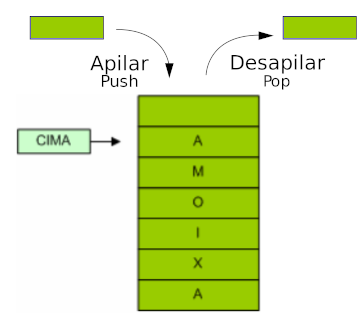
\includegraphics[width=0.6\textwidth]{resources/pila01.png}
        \caption{Definición gráfica de pila.}
        \label{pila01}
    \end{figure}

    \subsection{Operaciones sobre pila}
    
        Las operaciones básicas para el mantenimiento de una pila y de sus elementos se definen
        como:

        \begin{itemize}
            \item Inserción, apilación o push.
            \item Eliminación, desapilación o pop.
            \item Comprobación de pila vacía.
            \item Comprobación de pila llena (sólo para pila estática).
            \item Limpiar todos los elementos de la pila (pop).
            \item Obtención de tamaño máximo (sólo para pila estática).
            \item Obtención de cima (primer elemento de la pila).
        \end{itemize}

    \subsection{Implementación estática de pila}

        La implementación estática se basa en arrays, siendo éste usado como estructura de almacenamiento 
        de los elementos de la pila. Este array tiene que tener una dimensión prefijada\footnote{
            Cuando se sobrepasa el límite de almacenamiento de una pila se produce un error de 
            desbordamiento positivo, también denominado \textbf{overflow}.
            
            Por el contrario, cuando se intenta extraer un elemento inexistente de la pila, se producirá 
            un desbordamiento negativo, también denominado \textbf{underflow}.
        }, pues estamos 
        tratando una implementación estática.

        Los elementos de la pila se insertarán comenzando por la posición 1 del array y continuarán 
        insertándose en posiciones consecutivas. 

        \subsubsection{Declaración y definición de la pila}

            Ya que se basa en un array que almacena los elementos y un número que ejerce de índice 
            para indicar dínde se encuentra la cima de la pila, usaremos una estructrua como:

            \begin{lstlisting}[language=C,numbers=left]
    typedef struct 
    {
        TipoDato Elementos[10];
        int cima;
    } PilaEstatica; \end{lstlisting}

        \subsubsection{Creación de la pila}

            La creación se hace automáticamente cuando defininimos un tipo de dato de nuestra pila:

            \begin{lstlisting}[language=C,numbers=left]
    PilaEstatica p;\end{lstlisting}

            Siendo que consideramos una pila vacía cuando el índice que representa la cima tenga 
            el valor $-1$, una inicialización correcta de la pila debería añadir una inicialización 
            de su índice a este valor:

            \begin{lstlisting}[language=C,numbers=left]
    p->cima = -1;\end{lstlisting}

        \subsubsection{Inserción de elemento a la pila} % TODO

        \subsubsection{Vaciado de pila} % TODO

        \subsubsection{Obtención de elemento de la pila} % TODO

        \subsubsection{Obtención de total de elementos de la pila} % TODO

        \subsubsection{Comprobación de vaciado de pila} % TODO

        \subsubsection{Comprobación de llenura de pila} % TODO


    \subsection{Implementación dinámica de pila}

        Es una implementación dinámica de basada en \textbf{listas enlazadas} 
        (véase apartado \ref{listasenlazadas}). Tienen la particularidad de que todas 
        las inserciones y eliminaciones de elementos se realizarán por uno de los extremos
        de la lista (\textit{cima}).

        Este modo de implementación sólo utiliza la memoria necesaria en cada momento, puesto 
        que se reserva memoria para cada nuevo nodo que se inserta y se libera para cada nodo
        que se elimina. Por lo tanto no desperdicia memoria.

        Este modo de implementación no prefija ningún tamaño, como ocurre en la implementación 
        estática; la pila irá creciendo y decreciendo seún demando la aplicación que se hace de 
        ella.

        En este tipo de implementación no hay que controlar el \textit{overflow}, aunque si se 
        debe comprobar que el sistema pudo crear el nodo que se solicitó para insertar un nuevo 
        elemento en la pila. Es decir, que hay memoria suficiente añ hacer la reserva con las 
        funciones ya conocidas (\textit{malloc}, \textit{calloc} y \textit{realloc}).

        Técnicamente, la implementación dinámica de una pila es exactamente igual a la implementación 
        dinámica de una lista enlazada (véase apartado \ref{listasenlazadas}) simplemente añadiendo las 
        restricciones adecuadas.

\section{Colas}

    A las colas se accede de manera \textit{First in first out (FIFO)}, es decir, el primer 
    elemento en entrar es el primero en salir. Cabe destacar que en muchos textos se hace referencia 
    a las colas a través de su origen anglosajón \textbf{queque}.

    Una cola es pues, una colección de elementos homogéneos, llamados nodos, con una relación lineal 
    entre ellos ($a_i$ sucede a $a_{i-1}$) y a los que se accede por sus dos extremos.

    Un extremo se denomina \textbf{cabeza} o \textbf{frente} y es por donde se atiende a los elementos
    (o se eliminan); mientras que al otro extremo se le denomina \textbf{final} o \textbf{último}, y es 
    por donde se insertan nuevos elementos (véase figura \ref{cola01}).

    \begin{figure}[htp]
        \centering
        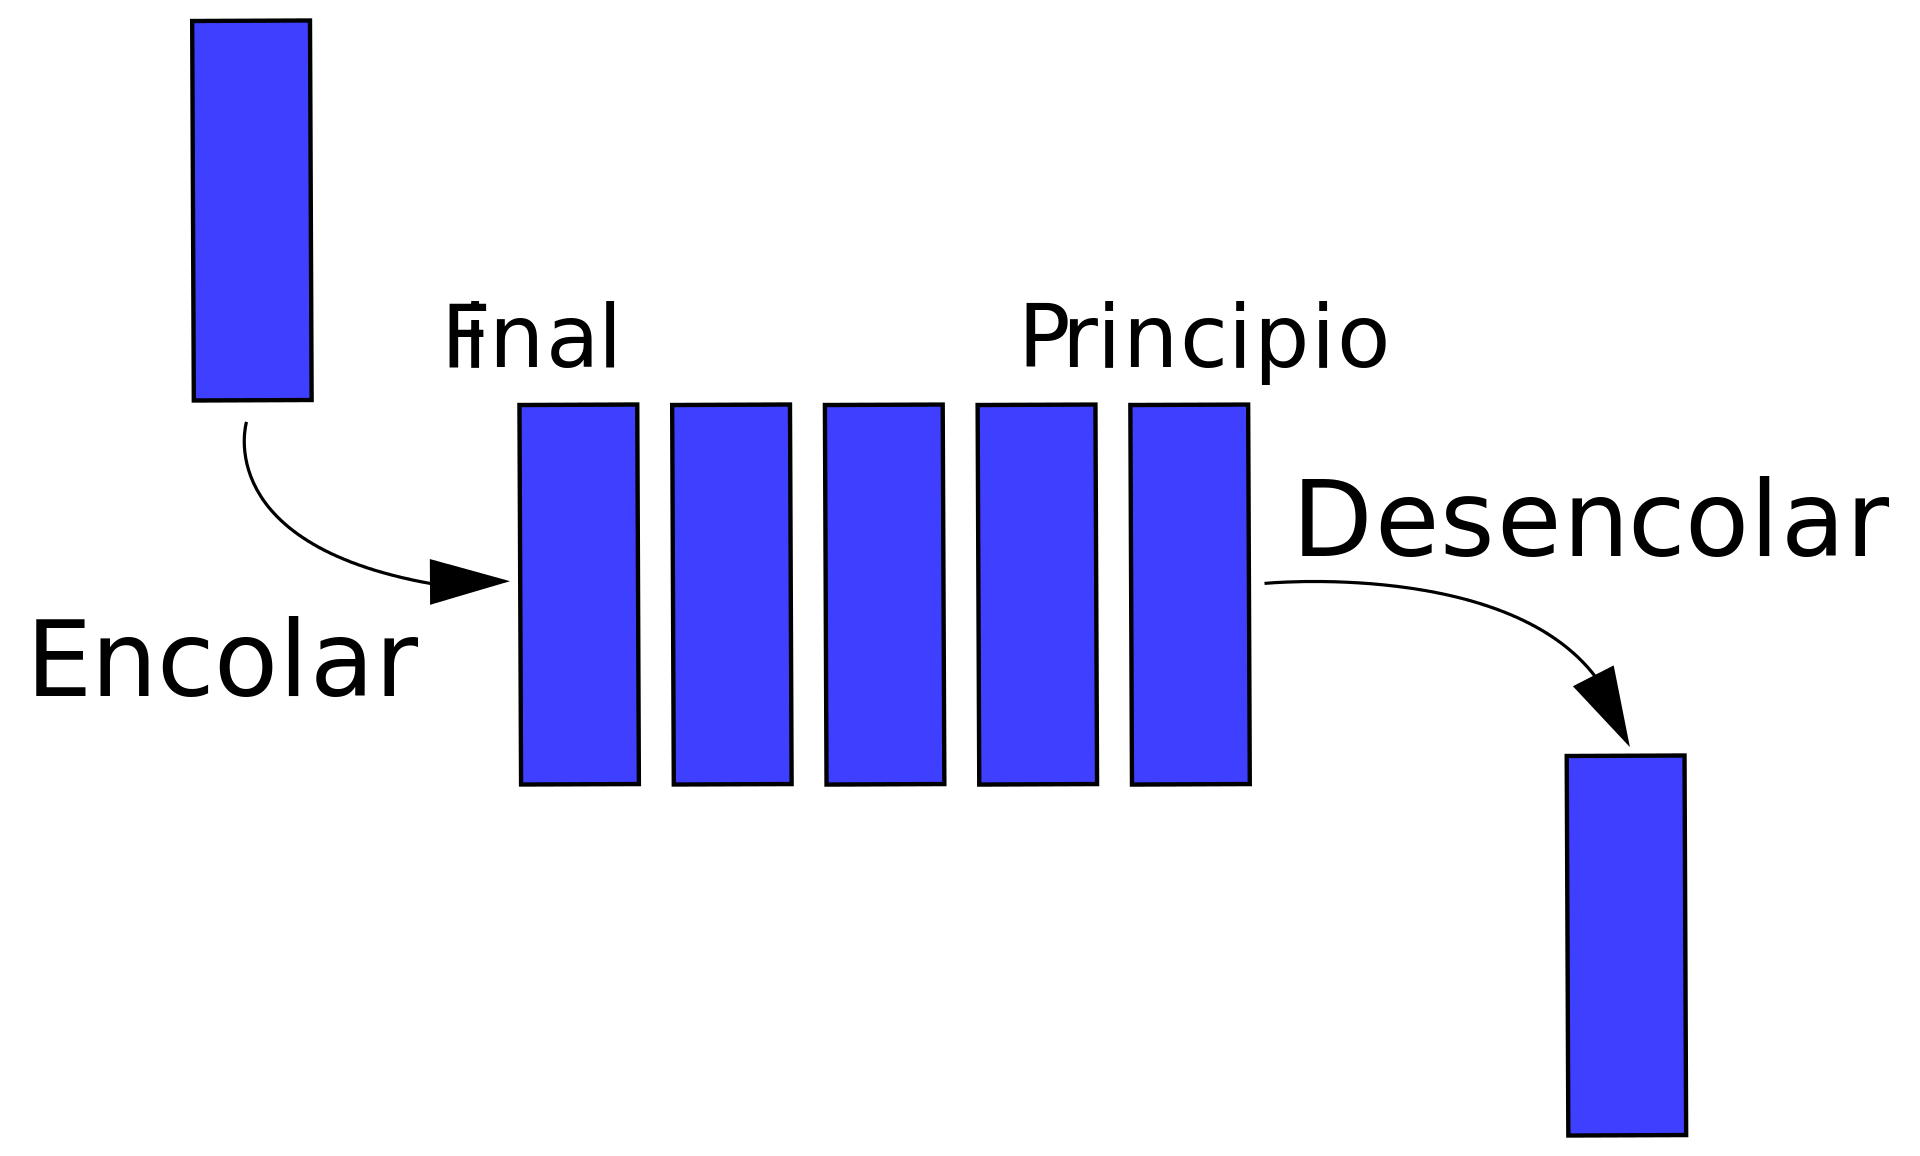
\includegraphics[width=0.6\textwidth]{resources/cola01.png}
        \caption{Definición gráfica de cola.}
        \label{cola01}
    \end{figure}

    \subsection{Implementación estática de cola}

        Las colas estáticas se caracterizan por los siguientes aspectos:

        \begin{itemize}
            \item Es una implementación basada en arrays. Usaremos un array a modo de estructura de 
            almacenamiento de los elementos d la cola.
            \item Es necesario definir su capacidad máxima (dimensión del array), puesto que estamos 
            trabajando con una implementación estática.
            \item Es necesario mantener dos índices numéricos. Uno indicando dónde se encuentra la cabeza 
            de la cola; y el otro dónde se encuentra el final de ésta.
        \end{itemize}

        Dentro de la implementación estática encontraremos dos variantes:

        \begin{itemize}
            \item Cola lineal
            \item Cola circular
        \end{itemize}

    \subsection{Implementación dinámica de cola}

        Las colas implementadas dinámicamente se caracterizan por estar basadas en las implementaciones 
        del tipo lista enlazada (véase apartado \ref{listasenlazadas}). Las operaciones no difieren mucho 
        de las ya estudiadas en éstas, considerándose una cola implementada dinámicamente como una 
        lista enlazada dinámicamente, pero con restricciones.

    \subsection{Casos especiales de colas}

        Existen algunas implementaciones de colas y conceptos que presentan peculiaridades en cuanto a su 
        estructura o forma de operar.
        
        \subsubsection{Bicola}

            Una bicola, o cola bidireccional se define como un caso especial de cola que permite 
            realziar tanto inserciones como eliminaciones por cualquiera de sus extremos indistintivamente.

        \subsubsection{Colas de prioridad}

            Se trata de una variante de cola que pretende que los elementos sean extraídos de ella según 
            una prioridad establecida (los prioritarios salen antes). Para lograr esto es lógico que cada 
            elemento de la cola debe tener una prioridad, y la inserción debe hacerse en función de ésta.

            Normalmente la prioridad se establece mediante un valor numérico; y cuando menor sea éste 
            mayor será su prioridad. A igualdad de prioridad entre los elementos, la extracción de la cola 
            se realizará en orden de llegada (funcionamiento genérico de las colas).

\section{Recursividad}

    \subsection{Recursividad teórica}

        La recursividad es una característica de los lenguajes de programación en los que se permite 
        que una función haga referencia a sí misma, invocándose, dentro de su propia implementación.

        En términos operacionales, la ejecución de una función recursiva genera una o más invocaciones 
        de la propia función, cada una de las cuales genera nuevas invocaciones y así sucesivamente.

        La definición recursiva debe estar ideada de modo que la cadena de invocaciones termine 
        en algún momento, es decir, con una llamada que no genere nuevas invocaciones (si no, tendremos 
        una cadena recursiva infinita e indefinida).
    
        \begin{figure}[htp]
            \centering
            
\includegraphics[width=0.3\textwidth]{resources/recursividad.jpg}
            \caption{Definición gráfica de recursividad.}
            \label{recursividad01}
        \end{figure}

        Una función recursiva debe cumplir dos propiedades:

        \begin{itemize}
            \item Debe tener una condición de la cual dependa la llamada recursiva y la salida de la 
            función. A esta condición se le denomina \textbf{condición de salida}.
            \item Debe modificar la condición de salida en cada llamada recursiva, de modo que exista 
            una aproximación cada vez mayor al caso base (salida). De lo contrario, caeríamos en 
            bucle infinito recursivo.
        \end{itemize}

        Se suele emplear la recursividad cuando la solución de un problema está expresada en términos 
        de un problema de igual naturaleza.

        Para que una función recursiva esté completamente definida es necesario tener un caso base 
        que no se calcule utilizando casos anteriores, y que la división del problema converja a este 
        caso base.

        \subsubsection{Ejemplo: cálculo del factorial con $n=3$}\label{factorial}

            Definición de la solución en términos de un caso base (el número 1), y otros casos 
            genéricos de la misma naturaleza que el problema; y menor tamañoque convergen hacia la 
            solución:

            \[
            n! = \begin{cases} 
            1 & \mbox{si } n = 0 \\ 
            n (n-1)! & \mbox{si }  n > 0 \end{cases}    
            \]
    
            En la figura \ref{factorial3} se muestran los pasos que se siguen en la ejeción de la solución recursiva 
            anterior.

            \begin{figure}[htp]
                \centering
                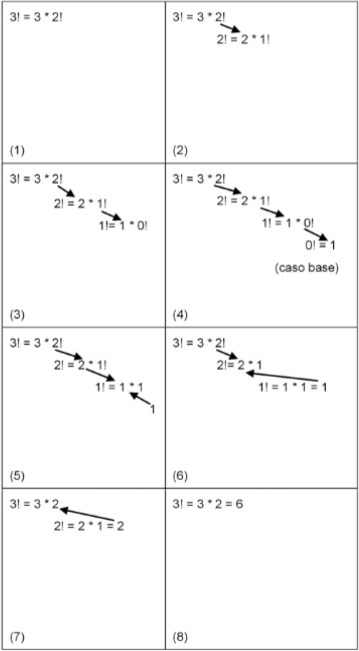
\includegraphics[width=0.4\textwidth]{resources/recursividad01.png}
                \caption{Secuencias de pasos de ejecución del cálculo del factorial de 3.}
                \label{factorial3}
            \end{figure}

    \subsection{Inducción y razonamiento inductivo}

        La inducción y el razonamiento inductivo son técnicas que nos van a ayudar a la hora de 
        diseñar algoritmos recursivos.

        \subsubsection{Inducción}

            La inducción es la técnica que se utiliza para demostrar enunciados matemáticos.

            Se compone de los siguientes pasos:

            \begin{itemize}
                \item Se parte de una afirmación para el caso más simple a estudiar o caso base.
                \item Si el enunciado es cierto para un determinado caso, entonces se debe verificar
                igualmente para el siguiente caso más complicado. A esta comprobación se e denomina 
                \textbf{Paso Inductivo}.
            \end{itemize}

            \paragraph{Ejemplo: suma de números naturales}

            Para un número $n>=0$ se verifica que:

            \[ 0 + 1 + 2 + ... + n = n (n+1)/2 \]

            Caso base: para $n=0$ tenemos que $0=0(0+1)/2$

            Paso inductivo:

            Suponiendo que el enunciado es verdadero para algún número $n$, entonces debe demostrarse si
            es cierto para $n+1$:

            \begin{equation}
                \begin{split}
                    &0 + 1 + 2 + ... + n + (n+1) \\
                    = &(n(n+1)/2) + (n+1) \\
                    = &(n2 + 3n + 2) / 2 \\
                    = &(n+1)(n+2)/2    
                    \nonumber
                \end{split}
            \end{equation}


    \subsection{Razonamiento inductivo}

        El razonamiento inductivo consiste en la obtención de conclusiones generales a partir de 
        premisas que contienen datos particulares. Por ejemplo, de la observación repetida de objetos 
        o acontecimientos de la misma índole se establece una conclusión para todos los objetos o 
        eventos de dicha naturaleza.

        Premisas:

        \begin{itemize}
            \item El perro $p_1$ tiene 4 patas.
            \item El perro $p_2$ tiene 4 patas.
            \item El perro $p_3$ tiene 4 patas.
        \end{itemize}

        Conclusión: \textbf{todos los perros tienen 4 patas}.

        La construcción de estos procedimientos no sigue una fórmula concreta, pero el programador 
        puede usar la noción de indución de la siguente forma:

        \begin{itemize}
            \item Solucionar el caso más simple. \textbf{Casoi base}.
            \item Expresar el caso general de la función de casos más simples que tiendan hacia el caso base.
            \item Desarrollar el algoritmo recursivo.
        \end{itemize}
        
        A continuación se muestra un ejemplo de aplicación del razonamiento inductivo al ejemplo tratado 
        anteriormente del cálculo del factorial de un número (véase apartado \ref{factorial}):

        \begin{lstlisting}[language=C,numbers=left]
    Funcion Factorial(n: entero): entero 
    var resultado: entero

    inicio
        Si (n=0)
            resultado = 1
        Si no
            // Llamada recursiva
            resultado=n + Factorial(n-1) 
            
            Devolver resultado
    Fin\end{lstlisting}

        Lo que daría una progresión de llamadas recursivas de la propia función, expresado gráficamente en
        la figura \ref{factorial4}.

        \begin{figure}[htp]
            \centering
            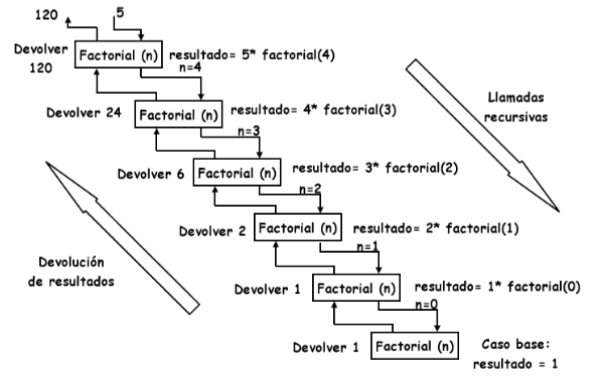
\includegraphics[width=0.8\textwidth]{resources/recursividad02.png}
            \caption{Progresión de llamadas recursivas expresadas gráficamente.}
            \label{factorial4}
        \end{figure}

    \subsection{Tipos de recursividad}

        Atendiendo a la forma que tenga elalgoritmo recursivo podemos hacer la siguiente 
        clasificación:

        \subsubsection{Recursividad lineal}

            Una llamada recursiva genera, como mucho, otra llamaad recursiva.

            \paragraph{Recursividad lineal por la cola} Es un tipo de recursividad lineal especial 
            en la que la llamada recursiva es la última operación que se realiza.

        \subsubsection{Recursividad múltiple}

            Son necesarias múltiples llamadas recursivas desde la misma función. Se distinguen 
            dos técnicas de recursividad múltiple:

            \paragraph{Técnica divide y vencerás}

                Consiste en transformar un problema de tamaño $n$ en problemas más pequeños, de tamaño 
                menor que $n$. De tal modo que dando solución a los problemas unitarios se pueda 
                cnstruir la solución al problema concreto.

                \subparagraph{Ejemplo: las Torres de Hanoi}

                    Hay tres postes: $A$, $B$ y $C$. En el poste $A$ se ponen $n$ discos de diámetro 
                    diferente detal manera que un disco de diámetro mayor siempre queda debajo de uno 
                    de diámetro menor. El objetivo es mover los discos al poste $C$ usando $B$ como
                    auxiliar. Sólo puede moverse un disco superior de cualquier poste a otro, y un disco 
                    mayor jamás puede quedar sobre uno menor.

                    \begin{figure}[htp]
                        \centering
                        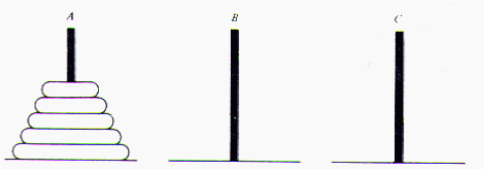
\includegraphics[width=0.7\textwidth]{resources/recursividad03.png}
                        \caption{Situación inicial en el problema de las Torres de Hanoi.}
                        \label{hanoi01}
                    \end{figure}
            
                    Si planteamos el problema con un solo disco, su solución es tan simple como mover 
                    el disco del poste $A$ al poste $C$.

                    Si planteamos el problema con dos discos, la solución implicaría mover el disco 
                    más pequeño de $A$ a $B$, el más grande de $A$ a $C$ y finalmente el disco pequeño 
                    de $B$ a $C$. Esta forma de operar es válida para cualquier número de discos $n$. 
                    Consistiría en mover los $n-1$ discos superiores de $A$ a $B$, el disco $N$ de 
                    $A$ a $C$ y, finalmente, los $n-1$ de $B$ a $C$. Con la particularidad recursiva de 
                    que el movimiento de los $n-1$ discos de un poste a otro es nuevamente el mismo 
                    problema de las Torres de Hanoi, pero con un disco menos (Véase la figura \ref{hanoi03}
                    para observar la secuencia de movimientos representada gráficamente).

                    \begin{figure}[htp]
                        \centering
                        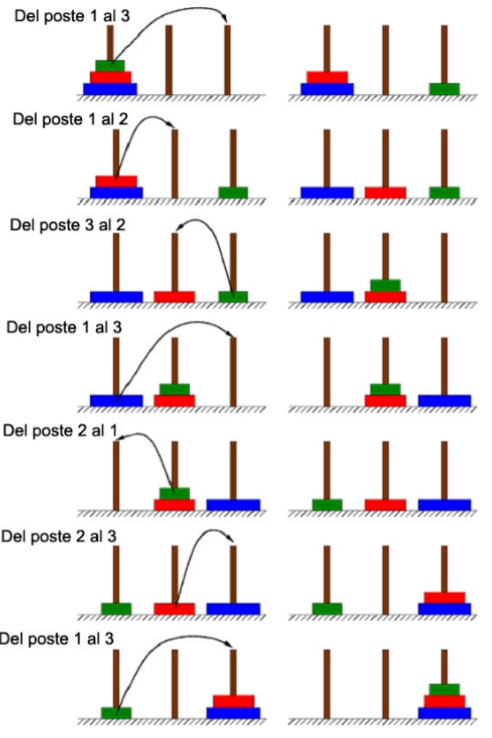
\includegraphics[width=0.7\textwidth]{resources/recursividad05.png}
                        \caption{Secuencia de movimientos para el problema de las Torres de Hanoi con 
                        3 discos.}
                        \label{hanoi03}
                    \end{figure}

            \paragraph{Técnica de vuelta atrás o backtracking}

                Los algoritmos de vuelta atrás se utilizan para encontrar soluciones a un problema 
                mediante la exploración de todas las posibilidades.

                No se siguen unas reglas refinadas para la búsqueda de la solución, simplemente una 
                búsqueda sistemática que más o menos viene a significar que hay que probar todos los 
                casos posibles hasta encontrar la solución, o en su defecto queno existe solución para 
                el problema.

                Para conseguir este propósito se separa la búsqueda en varias búsquedas parciales o 
                subtareas; así mismo, estas subtareas suelen incluir más subtareas (vemos pues la 
                recursividad).

                Puesto que a menudo nos interesa conocer todas las posibles soluciones a un problema, 
                estos algoritmos se pueden modificar fácilmente para obtner una sola solución o todas 
                las posibles.

                \subparagraph{Ejemplo: Recorrido del Caballo}

                    Se dispone de un tablero de ajedrez (de dimensión $8\times 8$) y de un caballo que 
                    se mueve siguiendo las reglas clásicas del juego. El objetivo es encontrar una manera 
                    de recorrer todo el tablero partiendo de una casilla determinada, de forma que el 
                    caballo pase una sola vez por cada casilla.

                    Para resolver el problema hay que realizr todos los movimientos posibles hasta que 
                    se cubra el tablero completo, o hasta que no se pueda avanzar más (en cuyo caso hay 
                    que dar marcha atrás).

                    El tablero será representado como una matriz $8\times 8$ de números enteros. Inicialmente 
                    todas las casillas contendrán el valor 0, indicando que no han sido visitadas aún.
                    Conforme el caballo pase por ellas su valor pasará a ser el número de movimiento en el 
                    que el caballo pasó por esa casilla.

                    Con las coordenadas de la casilla en las que se encuentre el caballo y las 8 coordenadas 
                    relativas de las casillas a las que puede moverse determinaremos los posibles movimientos.

                    Las coordenadas relativas las almacenaremos en dos arrays:

                    \begin{equation}
                        \begin{split}
                            ejex &= [2,1,-1,-2,-2,-1,1,2] \\
                            ejey &= [1,2,2,1,-1,-2,-2,-1]
                            \nonumber
                        \end{split}
                    \end{equation}

                    Así, a partir de una posición en la que se encuentre el caballo, sumándole a la 
                    coordenada $x$ de la posción, el primer valor de $ejex$ y a la coordenada $y$ el 
                    primer valor de $ejey$, obtendremos la posición correspondiente al movimiento 1.
                    El proceso es similar para el resto de movimientos, cambiando las posiciones de 
                    $ejex$ y $ejey$ que se suman a las coordenadas.

                    Cuando se encuentra una solución, una variable que se pasa por referencia es puesta 
                    a 1.

                    Es necesario indicar que para codificar la solución es necesario tener en cuenta 
                    otros factores, como controlar que no se salga de los límites del tablero o no 
                    pisar una casilla ya cubierta (selección del candidato).

                    Se determina que hay una solución cuando ya no hay más casillas que recorrer, es 
                    decir, se hayan realizado los 64 movimientos.

                    
                    \begin{lstlisting}[language=C,numbers=left,basicstyle=\small]
    #include <stdio.h>

    #define N 5
    #define ncuad N*N
    
    const int   ejex[8] = {-1,-2,-2,-1,1,2,2,1},
                ejey[8] = {-2,-1,1,2,2,1,-1,-2};
    
    
    void mover(int tablero[][N], int i, int pos_x, int pos_y, int *q)
    {
        int k,u,v;
    
        k = 0;
        *q = 0;
    
        do {
            u = pos_x + ejex[k];
            v = pos_y + ejey[k];
    
            if (u >= 0 && u < N && v >= 0 && v < N) {
                if (tablero[u][v] == 0) {
                    tablero[u][v] = i;
                    if (i < ncuad) {
                        mover(tablero, i+1, u, v, q);
                        if (!*q) tablero[u][v] = 0; 
                    }
                    else *q = 1;
                }
            }
            k++;
        } while (!*q & k < 8);
    }
    
    int main(void)
    {
        int tablero[N][N];
        int i,j,q;
    
        for (i = 0; i < N; i++)
            for (j = 0; j < N; j++)
                tablero[i][j] = 0;
    
        tablero[0][0] = 1;
        mover(tablero,2,0,0,&q);
    
        if (q)
        {
            for (i = 0; i < N; i++) {
                for (j = 0; j < N; j++)
                    printf("%3d", tablero[i][j]);
                putchar('\n');
            }
        }
        else 
            printf("\nNo existe solucion\n");
        return 0;
    }\end{lstlisting}
                    
    \subsection{Ventajas e inconvenientes de la recursividad}

        La recursividad, como es lógico presenta tanto ventajas como inconvenientes que hay que 
        tener en cuenta a la hora de implementar sistemas recursivos:

        Las principales \textbf{ventajas} que ofrece son:

        \begin{itemize}
            \item Permite la resolución de problemas de manera natural, sencilla y elegante.
            \item No es necesario definir la secuencia de pasos exacta para resolver el problema.
            \item Simplicidad de comprensión de los algoritmos.
            \item Reducción notable del tamaño del código.
        \end{itemize}

        Mientras que los principales inconvenientes o \textbf{desventajas} son:

        \begin{itemize}
            \item No siempre resulta fácil encontrar la solución recursiva a un problema.
            \item Son menos eficientes que las soluciones iterativas, tanto en consumo de memoria 
            como en velocidad. Esto es debido a que cada llamada recursiva implica una asignación 
            dinámica de memoria (de la zona conocida como Pila) y las sucesivas llamadas ralentizan 
            la ejecución.
            \item Algunos autores la tachan de confusa y peligrosa, puesto que puede llegar a agotar 
            los recursos de memoria del sistema.
        \end{itemize}

\section{Árboles}

    Un arbol es una colección de elementos homogéneos denominados nodos entre los que 
    existe una relación que impone una estructura jerárquica. Uno de los nodos se distingue
    siempre como raíz (\textit{root}) del árbol (véase figura \ref{arbol01}).

    \begin{figure}[htp]
        \centering
        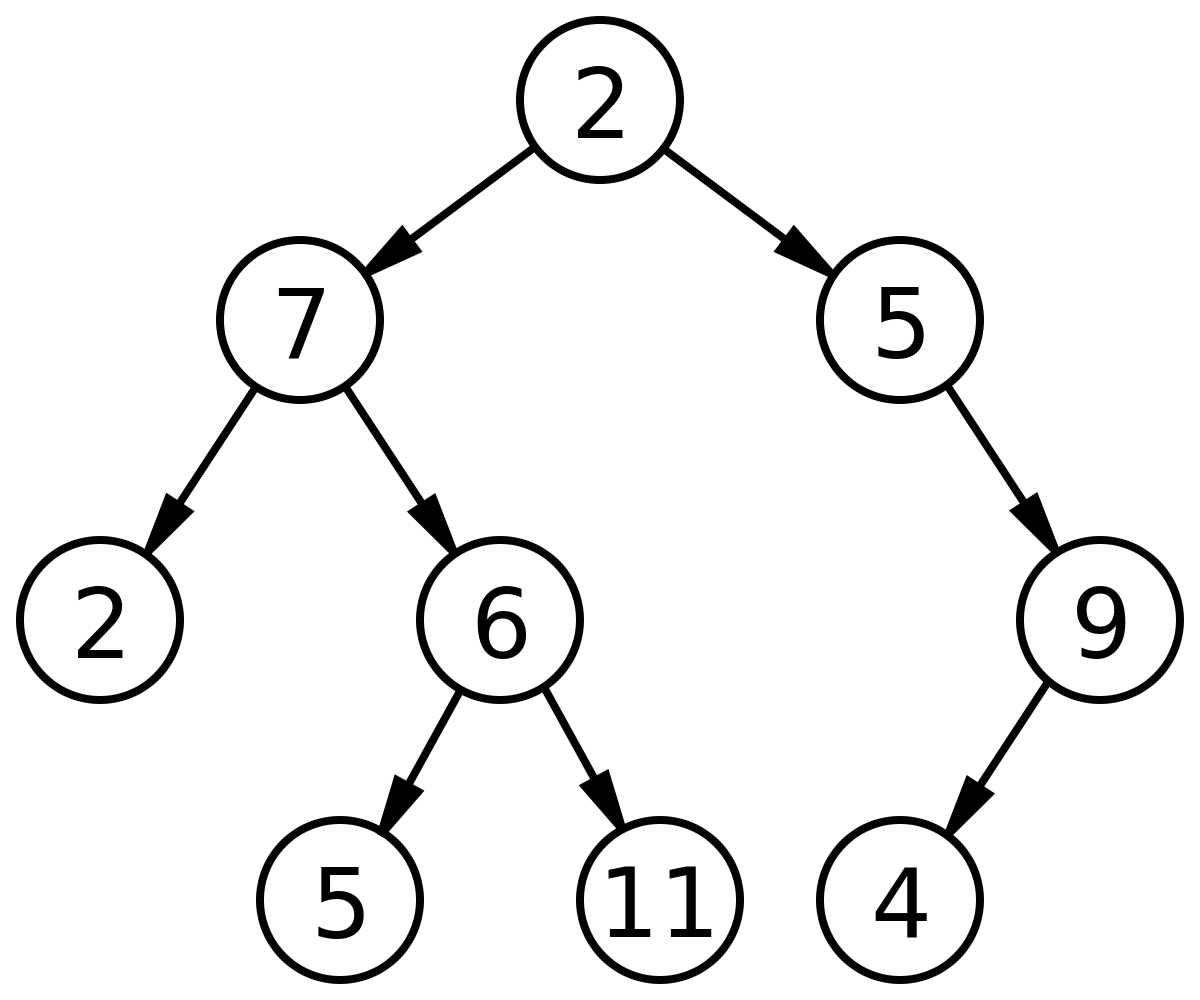
\includegraphics[width=0.4\textwidth]{resources/arbol01.png}
        \caption{Ejemplo de árbol binario.}
        \label{arbol01}
    \end{figure}

    \begin{enumerate}
        \item Hay un nodo especial ($n_1$) que es la raíz del árbol.
        \item Los nodos restantes ($n_2 ... n_m$) se dividen en $x$ conjuntos distintos, 
        con $x\geq 0$, llamados $t_1, t_2 ... t_x$. Tal que cada $T_i$ es por sí mismo un 
        árbol al que se le denomina subárbol. 
    \end{enumerate}

    Observamos pues la naturaleza recursiva del árbol. Cuando el número de nodos de un árbol
    es igual a 0 decimos que se trata de un árbol vacío o nulo. Podemos definir las propiedades 
    que definen esta estructura:

    \begin{itemize}
        \item Todo árbol que no está vacío, debe tener un único nodo raíz.
        \item Un nodo $x$ es descendiente directo de otro $y$ si existe una arista que va 
        desde $y$ a $x$. En este caso diremos que $x$ \textbf{es hijo} de $y$.
        \item Un nodo $x$ es antecesor directo de otro $y$ si existe una arista que va desde
        $x$ a $y$. En este caso diremos que $x$ \textbf{es padre} de $y$.
        \item Todos los nodos que son descendientes directos de un mismo nodo se denominan 
        \textbf{hermanos}.
        \item Cada nodo tiene que tener un número arbitrario de hijos, incluido 0.
        \item Todo nodo que no tiene hijos se denomina \textbf{hoja} o \textbf{terminal}.
        \item Todo nodo que no es hoja ni raíz es un \textbf{nodo interno}.
    \end{itemize}

    \subsection{Terminología teórica}

        Es necesario conocer la terminología empleada en el trabajo con estructuras de tipo 
        árbol:

        \paragraph{Grado de salida o grado de nodo} Número de descendientes directos de ese nodo.
         Así, el grado de un nodo hoja es 0.
        \paragraph{Grado de árbol} Grado máximo de todos sus nodos.
        \paragraph{Nivel o profundidad de nodo} Número de aristas que hay que recorrer para
        llegar al nodo desde la raíz. Así, el nivel de raíz es 0. Es posible organizar los árboles por 
        niveles, siendo el primero el nivel 0, luego el 1 y así sucesivamente.
        \paragraph{Altura de árbol} Número de niveles que tiene un árbol, o lo que es lo mismo, 
        número máximo de nivel de todos sus nodos $+1$. Se representa con la letra $H$.
        \paragraph{Camino de nodo $n_1$ a otro $n_k$} Secuencia de nodos $n_1, n_2 ... n_k$, 
        tal que $n_i$ es el padre de $n_{i+1}$ para $1\leq  i < k$
        \paragraph{Longitud de camino} Número de aristas que forman el camino o números de nodos 
        $-1$ que lo forman. Siempre hay un camino único entre la raíz y cualquier nodo y siempre existe 
        un camino de longitud 0 entre un nodo y él mismo. Siempre que exista un camino de un nodo
        $n_i$ a otro $n_j$; $n_j$ va a ser \textbf{descendiente} de $n_i$ y $n_i$ \textbf{antecesor}
        de $n_j$.
        \paragraph{Árbol ordenado} Un árbol se considera ordenado cuando sus nodos se encuentran 
        ordenados\footnote{
            El criterio que se sigue para ordenar los nodos es el siguiente: si $A$ y $B$ son hermanos,
            y $A$ está a la izquierda de $B$, todos los descendientes de $A$ están a la izquierda de todos
            los de $B$.
        } de izquierda a derecha.

    \subsection{Árbol Binario de Búsqueda (ABB)}

        Los árboles binarios son árboles de orden 2, es decir, cada nodo puede tener un máximo de 
        3 hijos (ó 0, ó 1, ó 2; véase figura \ref{arbol01}). Es uno de los tipos de árboles más usado, 
        pudiendo categorizarse según su finalidad.

        Un árbol binario con raíz $R$ va a ser de búsqueda cuando:

        \begin{itemize}
            \item No está vacío o null.
            \item Tiene un subárbol izquierdo $R_i$, donde $R_i < R$ y a su vez, $R_i$ también es
            de búsqueda, recursivamente.
            \item Tiene un subárbol derecho $R_d$, donde $R_d > R$ y a su vez, $R_d$ también es
            de búsqueda, recursivamente.
        \end{itemize}

        Véase la figura \ref{arbol02} para identificar un árbol de búsqueda; y la figura 
        \ref{arbol01} para identificar un árbol que no puede ser de búsqueda.

        \begin{figure}[htp]
            \centering
            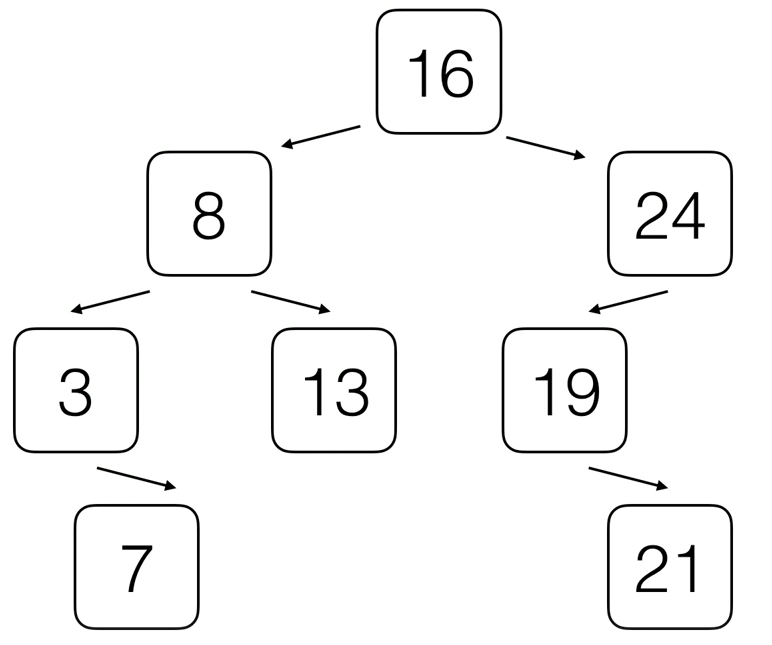
\includegraphics[width=0.4\textwidth]{resources/arbol02.png}
            \caption{Ejemplo de árbol binario de búsqueda.}
            \label{arbol02}
        \end{figure}

        Para que esto sea posible es necesario que los elementos almacenados en los árboles 
        de búsqueda cumplan una relación de orden; en otras palabras, sean comparables entre 
        sí (números enteros, cadenas de caracteres ordenadas por orden lexicográfico, objetos 
        identificables...).
    
        \subsubsection{Implementación de árbol binario de búsqueda}

            Una vez conocida la teoría, podemos comenzar con la implementación del árbol. 
            
            \paragraph{Declaración de estructura} Conociendo que un árbol se compone de subárboles podemos aprovecharnos de la 
            recursividad para desarrollar su estructura padre/hijo:

            \begin{lstlisting}[language=C,numbers=left]
    typedef struct nodo {
        int valor;
        struct nodo* izquierdo;
        struct nodo* derecho;
    } Nodo;
    
    typedef Nodo Arbol;\end{lstlisting}

            \paragraph{Creación de árbol y nodos} La creación de cada nodo es muy sencilla; en este caso estamos empleando un 
            árbol que almacena enteros \textit{valor}, por lo que simplemente definiremos 
            una función que cree el nodo mediante \textit{malloc} y asigne el valor 
            pasado. Como no tiene hijos al crearse, los nodos hijos derecho e izquierdo 
            quedarán a \textit{null}.

            \begin{lstlisting}[language=C,numbers=left]
    Nodo* CrearNodo(int valor) {
        Nodo* n = (Nodo *) malloc(sizeof(Nodo));
        n->valor = valor;
        n->derecho = n->izquierdo = NULL;
        return n;
    }
    Arbol *arbol = CrearNodo(10); // nodo con valor 10\end{lstlisting}

            \paragraph{Destrucción de nodo} Para destruir un nodo es tan sencillo como liberar el espacio con \textit{free}.
            Por si acaso asignaremos el valor \textit{null} a sus nodos hijos.

            \begin{lstlisting}[language=C,numbers=left]
    void DestruirNodo(Nodo* n) {
        n->derecho = n->izquierdo = NULL;
        free(n);
    }\end{lstlisting}

            \paragraph{Inserción de nodos en árbol} Como ya sabemos, cuando queremos insertar 
            un nodo, que es un árbol como hijo de otro lo situará a izquierda o derecha 
            dependiendo de la relación de orden. En este caso comprobando el orden numérico, 
            ya que estamos trabajando con valores enteros.
            
            \begin{lstlisting}[language=C,numbers=left]
    void Insertar(Nodo** arbol, int valor) {
        if (*arbol == NULL) {
            Nodo* n = CrearNodo(valor);
            *arbol = n;
        } else {
            // Los elementos menores a la izq, los elementos
            // mayores a la der.
            int valorRaiz = (*arbol)->valor;
            if (valor < valorRaiz) {
                Insertar(&(*arbol)->izquierdo, valor);
            } else {
                Insertar(&(*arbol)->derecho, valor);
            }
        }
    }\end{lstlisting}

            \paragraph{Búsqueda en árbol} Para realizar la búsqueda simplemente analizaremos 
            el valor del nodo/árbol pasado por parámetro y, en caso de no coincidir y en 
            función de la relación de orden se llamará recursivamente para ser introducido en 
            el hijo correspondiente. Así, hasta dar con él si existiera.

            \begin{lstlisting}[language=C,numbers=left]
    int Existe(Nodo* arbol, int valor) {
        if (!arbol) {
            return 0;
        } else if (arbol->valor == valor) {
            return 1;
        } else if (valor < arbol->valor) {
            return Existe(arbol->izquierdo, valor);
        } else {
            return Existe(arbol->derecho, valor);
        }
    }\end{lstlisting}

            \paragraph{Recorridos de árboles} Como hemos visto anteriormente, la necesidad de 
            visualizar o acceder al contenido de la infomación almacenada en un árbol implica tener 
            que moverse entre los nodos que conforman su estructura.

            En una estructura lineal resulta fácil y trivial establecer un criterio de movimiento 
            por la misma. Pero en un árbol esa tarea no es tan simple.

            La definición de recorrer para este caso es la de visitar todos los nodos del árbol, de tal 
            forma que cada uno sea visitado una única vez. Existen dos tipos de recorrido:

            \subparagraph{Recorridos en profundidad} Para el que existen tres métodos de naturaleza 
            recursiva, que imponen un orden secuencial y lineal sobre los nodos del árbol. Realizando 
            cada uno de estos métodos siempre las actividades:

            \begin{itemize}
                \item Visitar el nodo raíz.
                \item Recorrer el subárbol izquierdo.
                \item Recorrer el subárbol derecho.
            \end{itemize}

            Pero cada método se diferencia en el oden en el que llevan a cabo estas actividades:

            El método de recorrido \textbf{PreOrden} o \textbf{PreOrder} se caracteriza por visitar el 
            nodo raíz antes de recorrer el subárbol izquierdo y derecho, respectivamente:

            \begin{lstlisting}[language=C,numbers=left]
    void PreOrder(Nodo *3arbol) {
        if (arbol) {
            printf("%d,", arbol->valor);
            PreOrder(arbol->izquierdo);
            PreOrder(arbol->derecho);
        }
    }\end{lstlisting}

            El método \textbf{InOrden} o \textbf{InOrder} primero recorre el subárbol izquierdo, después 
            visita el nodo raíz y finalmente recorre el subárbol derecho:

            \begin{lstlisting}[language=C,numbers=left]
    void InOrder(Nodo *arbol) {
        if (arbol) {
            InOrder(arbol->izquierdo);
            printf("%d,", arbol->valor);
            InOrder(arbol->derecho);
        }
    }\end{lstlisting}

            El método \textbf{PostOrden} o \textbf{PostOrder} recorre primero los subárboles izquierdo 
            y derecho respectivamente, para después visitar el nodo raíz:

            \begin{lstlisting}[language=C,numbers=left]
    void PosOrder(Nodo *arbol) {
        if (arbol) {
            PosOrder(arbol->derecho);
            PosOrder(arbol->izquierdo);
            printf("%d,", arbol->valor);
        }
    }\end{lstlisting}
            
            Viendo la figura \ref{arbol03} podemos realizar un ejemplo de los 3 métodos de recorrido en profundidad.

            \begin{figure}[htp]
                \centering
                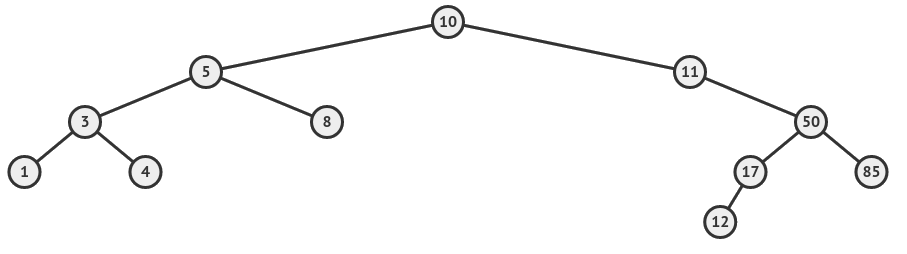
\includegraphics[width=1\textwidth]{resources/arbol03.png}
                \caption{Ejemplo de árbol binario de búsqueda para mostrar ejemoplos de recorridos.}
                \label{arbol03}
            \end{figure}

            Obteniendo los resultados: 

            \begin{itemize}
                \item Recorrido PreOrder: $10,5,3,1,4,8,11,50,17,12,85$
                \item Recorrido InOrder: $1,3,4,5,8,10,11,12,17,50,85$
                \item Recorrido PostOrder: $85,12,17,50,11,8,4,1,3,5,10$
            \end{itemize}

            El uso de uno u otro método ed recorrido en profundidad responde a las necesidades y 
            restricciones impuestas por el problema que se trata de resolver, no obstante es común usar
            cada recorrido en:

            \begin{itemize}
                \item PreOrder: en bases de datos con estructuras jerárquicas.
                \item InOrder: en búsquedas secuenciales.
                \item Para la evaluación y tratamiento de expresiones aritméticas.
            \end{itemize}

            \subparagraph{Recorrido en amplitud, anchura o por niveles} Este método consiste en comenzar 
            desde el nivel $i=0$ hasta la altura $h$ del árbol, visitando de izquierda a derecha los nodos 
            de profundidad $i$.

            Como observamos, un nodo $n_1$ aparece antes 
            que $n_2$ en el listado por niveles, si la 
            profundidad de $n_1$ es menor que la profundidad de $n_2$, y usando el orden de los nodos definido 
            (de izquierda a derecha), en caso de que tengan la misma profundidad.

            En el caso de la figura \ref{arbol03} el resultado obtenido tras un recorrido de este tipo 
            sería:

            \[ 10, 5, 11, 3, 8, 50, 1, 4, 17, 85, 12 \]

            Su implementación, debido a que no se basa en las relaciones padre-hijo no se puede hacer de forma 
            recursiva.

            % TODO Código implementación.

        \subsubsection{Árbol Binario de Busqueda Equilibrado o Balanceado}

            Es un árbol binario de búsqueda en el que para cada nodo se cumple que la altura del subárbol 
            derecho y la del izquierdo difieren como máximo en una unidad. Son árboles por lo tanto con 
            la necesidad de \textbf{mantenerlos equilibrados siempre}; si una operación de inserción o 
            eliminación que lo desequilibra, éste se reagrupa para lograr su equilibrio. Esto garantiza 
            que el árbol tendrá siempre la altura mínima y, por lo tanto, el \textbf{esfuerzo de búsqueda 
            será menor}.

            Este tipo de árboles también reciben el nombre de\textbf{árboles A.V.L.}, en honor a sus creadores 
            \textit{Adelson, Velskii y Londis}.

            % TODO Continuación arboles AVL

\end{document}